\documentclass[12pt,preprint]{aastex}
\usepackage{lsst}
\usepackage{xspace}
\usepackage[english]{babel}
\usepackage[utf8x]{inputenc}
\usepackage{hyperref}
\usepackage{amsmath}
\usepackage{graphicx}
\usepackage{longtable}
\usepackage{comment}
\usepackage{booktabs}

\newcommand{\Alert}{\code{Alert}\xspace}
\newcommand{\Alerts}{\code{Alerts}\xspace}
\newcommand{\DIASource}{\code{DIASource}\xspace}
\newcommand{\DIASources}{\code{DIASources}\xspace}
\newcommand{\DIAObject}{\code{DIAObject}\xspace}
\newcommand{\DIAObjects}{\code{DIAObjects}\xspace}
\newcommand{\DB}{{Level 1 database}\xspace}
\newcommand{\DR}{{Level 2 database}\xspace}
\newcommand{\Object}{\code{Object}\xspace}
\newcommand{\Objects}{\code{Objects}\xspace}
\newcommand{\Source}{\code{Source}\xspace}
\newcommand{\Sources}{\code{Sources}\xspace}
\newcommand{\ForcedSource}{\code{ForcedSource}\xspace}
\newcommand{\ForcedSources}{\code{ForcedSources}\xspace}
\newcommand{\CoaddSource}{\code{CoaddSource}\xspace}
\newcommand{\CoaddSources}{\code{CoaddSources}\xspace}
\newcommand{\SSObject}{\code{SSObject}\xspace}
\newcommand{\SSObjects}{\code{SSObjects}\xspace}
\newcommand{\VOEvent}{\code{VOEvent}\xspace}
\newcommand{\VOEvents}{\code{VOEvents}\xspace}
\newcommand{\transSNR}{5\xspace}


\begin{document}
\title{The Large Synoptic Survey Telescope as a Near-Earth Object Discovery Machine}

\author{R. Lynne Jones$^1$, Colin Slater$^1$, Joachim Moeyens$^1$,
Lori Allen$^2$, Mario Juri\'{c}$^1$,  \and \v{Z}eljko Ivezi\'{c} $^1$}

\affil{
$^1$University of Washington, \\
$^2$National Optical Astronomy Observatory}

\begin{abstract}
We discuss the ability of LSST to contribute to Near-Earth Objects (NEO) discoveries and
the Congressional George E. Brown, Jr. mandate to NASA. The two main issues addressed
here are the robustness of the LSST strategy for discovering NEOs using nightly pairs of
observations, and the expected cumulative completeness for potentially hazardous asteroids
(PHAs) with visual absolute magnitudes $H<22$.  We argue that the observing and data
processing strategies chosen by LSST are robust, and would yield a completeness of about
75\% for PHAs with $H<22$, using the current LSST baseline survey strategy (and assuming
no known objects prior to the survey). We describe in detail a number of modifications of the
LSST baseline survey which potentially could raise the completeness for PHAs with $H<22$
to 90\%. For example, with LSST baseline survey strategy extended to a 12-year survey,
the completeness for PHAs with $H<22$ becomes 86\%, with known objects taken into
account. We also discuss a number of systematic effects that must be taken into account
when comparing different simulations of the same survey, as well as simulations of different
surveys and observing systems.
\end{abstract}

\keywords{Near-Earth objects --- Image processing -- Asteroids}


\section{Introduction}

The small-body populations in the Solar System, such as asteroids, trans-Neptunian objects (TNOs)
and comets, are remnants of its early assembly. Collisions in the main asteroid belt between Mars and
Jupiter still occur, and occasionally eject objects on orbits that may place them on a collision course
with Earth. About 20\% of this near-Earth Object (NEO) population pass sufficiently close to Earth orbit such that
orbital perturbations with time scales of a century can lead to intersections and the possibility of collision. These objects that pass within 0.05 AU of Earth's orbit are termed potentially hazardous asteroids (PHAs).
In order to improve quantitative understanding of this hazard, in December 2005 the U.S. Congress
directed\footnote{National Aeronautics and Space Administration Authorization Act of 2005 (Public Law 109-155), January 4, 2005, Section 321, George E. Brown, Jr. Near-Earth Object Survey Act} NASA to implement a NEO survey that
would catalog 90\% of NEOs with diameters larger than 140 meters by 2020 (known as the George
E. Brown, Jr.\ mandate). It is estimated that there are about 30,000 such objects \citep{harris15}, with around 7,500 currently known.
For a compendium of additional information about NEOs and PHAs and an up-to-date summary of
discovery progress, see NASA's NEO webpage\footnote{\url{http://neo.jpl.nasa.gov/neo/}}.

The completeness level set by the Congressional mandate could be accomplished with a 10-meter-class
ground-based optical telescope, equipped with a multi-gigapixel camera and a sophisticated and robust data
processing system \citep[see NASA-commissioned reports by ][]{stokes03,shapiro10}. The Large Synoptic Survey Telescope\footnote{www.lsst.org} (LSST), currently being
constructed, is such a system. A concise LSST system description, discussion of science drivers, and other
information, are available in \cite{LSSToverview}. The LSST baseline strategy for discovering Solar System
objects is predicated on two observations of the same field per night, spaced by a few tens of minutes, and
a revisit of the same field with another pair of observations within a few days. The main reason for two
observations per night is to help association of observations of the same object from different nights,
as follows. The typical distance between two nearby asteroids on the Ecliptic, at the faint fluxes probed by
LSST, is a few arcminutes (counts are dominated by main-belt asteroids). Typical asteroid motion
during several days is larger (of the order a degree or more) and thus, without additional information,
detections of individual objects are ``scrambled''. However, with two detections per night, the motion
vector can be estimated. The motion vector makes the linking problem much easier because
positions from one night can be approximately extrapolated to future (or past) nights. The predicted
position's uncertainty is typically of the order of several arcminutes, rather than a degree, which effectively
``de-scrambles'' detections from different nights (for a detailed discussion of this algorithm, see
Appendix~\ref{sec:appMOPS}).

Early simulations of LSST performance presented by \cite{IvezicNEO2007} showed that the 10-year baseline
cadence would result in 75\% completeness for PHAs greater than 140 m (more  precisely, for PHAs with
$H<22$; see \S\ref{sec:GMS} for further discussion). They also suggested that with additional optimization of the
observing cadence, LSST could achieve 90\% completeness. An example of such an optimization was discussed
by \cite{LSSToverview} who reported that, to reach 90\% completeness, about 15\% of observing time would
have to be dedicated to NEOs, and the survey would have to run for 12 years.
%% From the overview paper:
%% - the LSST baseline cadence provides orbits for 82% of PHAs larger than 140 meters after 10 years of operations
%% - 84% completeness with minor changes to the cadence (5% of time for NEO-optimized observations)
%% - 90% completeness with major changes to the cadence (15% of time for NEO-optimized observations and 12 years)
The latest LSST simulation results, presented here, yielded a completeness of $\sim$68\% for
PHAs with $H<22$, using the current 10-year baseline survey. The minor differences in reported completeness
compared to older LSST studies are attributable to differences in simulated NEO populations and other modeling
details (such as improved hardware understanding).

These completeness estimates are based on an implicit assumption that 3 pairs of observations
obtained within a 15-30 day wide window are sufficient to recognize that these observations belong
to the same object, and to estimate its orbital parameters (the same criterion has been used in NASA
studies\footnote{See \url{http://neo.jpl.nasa.gov/neo/report2007.html}}).
This so-called linking of individual detections into plausible orbital tracks
will be performed using a special-purpose code referred to as the Moving Object
Processing System (MOPS). MOPS and its algorithms are significantly more
advanced than anything previously fielded for this purpose \citep{denneau13}. 

The described LSST strategy for discovering moving objects has been questioned (e.g., \citealt{GMS2016}) on
two grounds:
\begin{itemize}
\item A large number of false detections due to problems with image differencing software may
make linking problem prohibitively hard for MOPS. In particular, this objection is motivated by the experience
from extant surveys, such as Pan-STARRS and the Catalina Sky Survey.
\item Modifications of LSST baseline cadence, including image depth, sky coverage and cadence,
required to reach 90\% completeness level, have not yet been explicitly demonstrated using detailed
operations simulations, and made available to the community.
\end{itemize}
We aim to address these critiques here: the two major questions addressed by our study can be informally
stated as ``Will MOPS work?'' and ``If MOPS works, what fraction of  NEOs will LSST discover?''.

We use a combination of sophisticated simulations and real datasets to address these questions.
The main analysis components presented here include:
\begin{enumerate}
\item Analysis of the performance of prototype LSST image differencing software, with emphasis on the rate and
    properties of false detections (so-called ``false positives''), using DECam imaging data.
\item Analysis of the linking of asteroid detections in the presence of a large number of false positives, using MOPS
         and simulated observations.
\item Analysis of a large number of modified observing cadence simulations, coupled with NEO population
          models, to forecast discovery rates.
\end{enumerate}

We demonstrate that i) MOPS can cope with the anticipated false detection rates
in LSST difference images, and that ii) the NEO discovery performance of the LSST baseline cadence
can be appreciably boosted by adequate modifications of the observing strategy.
In \S2 we provide a brief overview of LSST and its strategy for discovering moving Solar
System objects. We discuss the performance of prototype LSST image differencing pipeline
in \S3, and MOPS performance in \S4. Modifications of the baseline cadence designed to
boost NEO/PHA completeness are described in \S5, and our results are summarized and
discussed in \S6.



\section{LSST Strategy for Discovering Solar System Objects} 

We briefly describe LSST design and observing strategy, and discuss in more
detail image processing and moving object detection. 


\subsection{Brief Overview of LSST  Design} 

LSST will be a large, wide-field ground-based optical telescope system
designed to obtain multiple images covering the sky that is visible
from Cerro Pach\'{o}n in Northern Chile. The current baseline design,
with an 8.4m (6.7m effective) primary mirror, a 9.6 deg$^2$ field of
view, and a 3.2 Gigapixel camera, will allow about 10,000 square
degrees of sky to be covered every night, with typical 5$\sigma$ depth 
for point sources of $r\sim24.5$ (AB). The system is designed to yield 
high image quality (the median delivered seeing in the $r$ band of 
about 0.8 arcsec) as well as superb astrometric  and photometric 
accuracy\footnote{For detailed specifications, please see the LSST
Science Requirements Document, http://ls.st/srd}. The total survey
area will include $\sim$30,000 deg$^2$ with $\delta<+34.5^\circ$, and 
will be imaged multiple times in six bands, $ugrizy$, covering the 
wavelength range 320--1050 nm. The project is scheduled to  begin the 
regular survey operations at the start of next decade. 

The LSST will be operated in fully automated survey mode. About 90\% of the 
observing time will be devoted to a deep-wide-fast survey mode which will 
uniformly observe a 18,000 deg$^2$ region about 1000 times (summed over 
all six bands) during the anticipated 10 years of operations, and yield a coadded map 
to $r\sim27.5$. These data will result in catalogs including about
$40$ billion stars and galaxies, that will serve the majority of the
primary science programs. The remaining 10\% of the observing time
will be allocated to special projects such as a Very Deep and Fast
time domain survey\footnote{Informally known as ``Deep Drilling Fields".}.



\subsection{LSST Observing Strategy} 

As designed and funded (by the U.S National Science Foundation and
Department of Energy), LSST is primarily a science-driven mission. 
The LSST is designed to achieve goals set by four main science themes:
\begin{enumerate}
\item Probing Dark Energy and Dark Matter;
\item Taking an Inventory of the Solar System;
\item Exploring the Transient Optical Sky;
\item Mapping the Milky Way.
\end{enumerate}
Each of these four themes itself encompasses a variety of analyses, with 
varying sensitivity to instrumental and system parameters. These themes 
fully exercise the technical capabilities of the system, such as photometric 
and astrometric accuracy and image quality. 

Existing cadence is optimized to maximize the overall science returns, including 
Solar System science, rather than NEO/PHA discovery completeness (though the 
two goals are highly interrelated). Discovering and linking objects in the Solar System 
moving with a wide range of apparent velocities (from several degrees per day for 
NEOs to a few arc seconds per day for the most distant TNOs) places strong 
constraints on the cadence of observations. The baseline cadence requires closely 
spaced pairs of observations, two or preferably three times per lunation. The visit
exposure time is set to 30 seconds to minimize the effects of trailing for the majority of 
moving objects. The images are well sampled to enable accurate astrometry, with 
anticipated absolute accuracy of at least 0.1 arcsec.

LSST observations can be simulated using the Operations Simulator tool (OpSim, XXX give
reference here). OpSim runs a survey simulation with given science-driven desirables; 
a software model of the telescope and its control system; and models of weather and other 
environmental variables. The output of such a simulation is an ``observation history'', which 
is a record of times, pointings and a record of associated environmental data and telescope  
activities throughout the simulated  survey.  This history can be examined to assess  
whether the simulated survey would be useful for any particular purpose or 
interest\footnote{For examples of such analysis, see http://ops2.lsst.org:8080 XXX shorten this URL!}. 


\subsection{LSST Baseline Cadence}

As the system understanding improves, the baseline cadence gets updated every few
years. The current baseline cadence is known as {\it minion\_1016}. It includes 2.4
million visits collected over 10 years, with 85\% of the observing time spent on the 
main survey and the rest on various specialized programs. The median number of visits
{\it per night} is 816, with 3,026 observing nights. The median airmass is 1.23 (the
minimum altitude for LSST telescope if 20 deg.). In the $r$ band, the median seeing 
(FWHM) is 0.81 arcsec, and the median $5\sigma$ depth for point sources is 24.16 
(using the best current estimate of the fiducial depth at airmass of one of 24.39). 

There are a few known problems with this simulation, including twilight sky brightness
estimates that are too bright, the moon avoidance is not as aggressive as it could be,
and observations are biased towards west, away from the meridian. An improved 
simulation will become available by the end of 2017. 

The performance of this simulated cadence in NEO context is discussed in detail in \S5. 


\subsection{Overview of LSST  Data Management and Image Processing} 

The images acquired by the LSST Camera will be processed by LSST Data Management
software \cite{juric15} to a) detect and characterize imaged
astrophysical sources and b) detect and characterize temporal changes
in the LSST-observed universe. The results of that processing will be
reduced images, catalogs of detected objects and their measured properties, and 
prompt alerts to ``events'' -- changes in astrophysical scenery discovered by differencing 
incoming images against older, deeper, images of the sky in the same direction ({\em
templates}). More details about the main algorithms and pipeline design are available
in Appendix~\ref{sec:AppA}. 

LSST will use two methods to detect moving objects in difference images: 
\begin{enumerate}
\item Detecting trailed motion on the sky: objects trailed by more
  than 2 PSF widths (corresponding to motion faster than about 1
  deg/day) will be easily detectable as trailed.  Two trailed
  detections within 30--60 minutes in a single night will be
  sufficient to identify an object as an NEO candidate,
\item Inter-night linking of pairs: this technique will recover
  objects moving too slow enough to be measurably elongated in 
  a single exposure. 
\end{enumerate} 


Sources detected in difference images (DIASources in LSST parlance, see Appendix~\ref{sec:AppA})
will include false detections, colloquially known as {\it false positives}. 



\section{Analysis of Image Differencing Performance \label{sec:imDiff}}

LSST will detect motion and flux variability by differencing each incoming image
against a deep template (built by combining multiple images of the same region).
Sources in difference images, called \DIASources, will be detected at a signal-to-noise
ratio (SNR) threshold of $\nu=5$. Up to about 1,000 deg$^{-2}$
astrophysical, real, detections (e.g. variable stars) are expected in LSST image differencing, including
up to about 500 deg$^{-2}$ asteroids on the Ecliptic. In addition to real detections,
there are false detections due to imaging or processing artifacts and 
false detections caused simply by statistical noise
fluctuations in the background. In a typical LSST difference image, the expected
density of false detections due to background fluctuations is about 60 deg$^{-2}$
(see below for details)---much lower than the expected rate of astrophysical
detections (see \S\ref{sec:kaiser} below). 

However, historically surveys have reported detection rates in image differencing that are much
higher, depending on the survey; see \cite{denneau13}; \cite{kessler15}; \cite{goldstein15}.
For example, Pan-STARRS1 (PS1) reported a transient detection rate as high as 8,200 deg$^{-2}$
\citep{denneau13}. For a ``menagerie'' of PS1 artifacts (with memorable names such as
{\it chocolate chip cookies, frisbee, piano, arrowhead, UFO}), see Fig.~17 in \cite{denneau13}.
They reported that ``Many of the false detections are easily explained as internal reflections,
ghosts, or other well-understood image artifacts, ...''. As discussed in \S\ref{sec:tracklets},
such a high false detection rate is at the limit of what could be handled even
with the substantial computing power planned for LSST.

Fortunately, Pan-STARRS1 was only a first-generation experiment and, over the past decade,
subsequent surveys have learned tremendously from the PS1 experience. There are surveys
running today, such as Dark Energy Survey, which have largely solved the key problems that
PS1 has encountered. Major improvements to hardware include CCDs with significantly fewer
artifacts (e.g. DECam, see below; LSST) and optical systems designed to minimize ghosting
and internal reflections (e.g. LSST). Improvements to the software include advanced image
differencing pipelines (e.g., PTFIDE for the Palomar Transient Factory and the Zwicky Transient
Facility) and various machine-learning classifiers for filtering false detections. For example,
\cite{goldstein15} used a Random Forest classifier with the Dark Energy Survey data
and cleaned their sample of transient detections from a raw false:true detection
rate ratio of 13:1 to a filtered rate of 1:3. The resulting false detections are
morphologically much simpler; for example, compare
Fig.~1 in \cite{goldstein15} to Fig.~17 in \cite{denneau13}.

Here we summarize an analysis of image differencing performance based on DECam
data and difference images produced and processed using prototype LSST
software \citep{DMTN-006}. This analysis demonstrates that the false
detection rate anticipated for LSST (without using any machine-learning classifiers for
filtering false positives) is significantly below the threshold for
successful deployment of MOPS, as will be discussed in \S\ref{sec:mops}.



\subsection{LSST Image Differencing Pipeline and Data Processing}

The LSST prototype image differencing and analysis code largely derives from the
HOTPANTS package \citep{becker15}, and was used for surveys such as SuperMACHO
\citep{becker05} and ESSENCE \citep{miknaitis07}. While this software is
functional as-is, it is expected that the ultimate LSST pipeline will include
improved methods for handling observations at high airmass and the effects of
differential chromatic refraction due to the Earth's atmosphere. Nevertheless, in
this work we conservatively assume that the pipeline used for LSST will have the
same performance as the current code.


\subsection{False Detections due to Background Fluctuations \label{sec:kaiser}}

Some false detections are expected simply due to background fluctuations, even
at a high SNR threshhold. The number of
such detections, as a function of the threshold SNR, the number of pixels and
seeing, can be computed using the statistics of Gaussian random fields.
For an image with a Gaussian background noise, convolved with a Gaussian point
spread function (PSF) with width $\sigma_g$ (in pixels), the number of peaks, $N$, above a
given SNR threshold, $\nu$, is given by (N. Kaiser, priv. comm.)
\begin{equation}
N(>\nu)  = \frac{n_{row}*n_{col}}{2^{5/2} \, \pi^{3/2} \, \sigma_g^2} \, \nu \, e^{-\nu^2 /2}
\label{eq-theory}
\end{equation}
where $n_{row}$ and $n_{col}$ are the number of pixel rows and columns in the image.
This expression was verified empirically by LSST data management team using
image simulations\footnote{See \url{https://github.com/lsst/W13report}}.
For 4k by 4k LSST sensors the pixel size is 0.2 arcsec, and for a nominal seeing
of 0.85 arcsec and $\nu=5$, $N(>\nu) = 59$ deg$^{-2}$.

It is generally not well appreciated just how steep is the dependence of $N(>\nu)$
on $\nu$ due to the exponential term. Changing the threshold from 5 to 5.5
decreases the expected rate by a factor of 12, and the rate increases by a factor
of 9.7 when the threshold is changed from 5 to 4.5. In practice, an empirical estimate
of the background noise is used when computing the SNR for each detected source.
When this estimate is incorrect, e.g. due to reasons discussed below, then the
implied detection threshold is wrong, too. For example, if the noise is underestimated
by only 10\%, the computed SNR will be too large by 10\%, and the adopted
threshold $\nu=5$ will actually correspond to $\nu=4.5$ -- and thus the
sample will include 9.7 times as many false detections due to background
fluctuations! Hence, the noise in difference images has to be estimated to
high accuracy.


\subsubsection{The Impact and Treatment of Correlated Noise}

When the LSST pipeline convolves the science image to match the PSF of the template
image, the per-pixel variance in the image is reduced, and at the same
time correlations between neighboring pixels are introduced. This violates the
assumption made by standard image processing algorithms that each pixel is an
independent draw from a Poisson distribution. The per-pixel noise reduction is
reflected in the variance plane that accompanies each exposure during
processing, but the covariance between pixels is not tracked.
The significance of detections and the uncertainties on source measurements is
then estimated based on this incomplete information provided by the variance
plane, leading to a biased detection threshold.

The magnitude of this effect can be large---using only the per-pixel variance
measurements can result in underestimating the true noise on PSF-size scales by
20\% or more. A detection threshold of $\nu=5$ thus actually corresponds to
$\nu=4$, and it is easy to see using eq.~\ref{eq-theory} that this error results
in an increase in the number of false positives by a factor of $\sim$70!

A histogram of the number of sources detected in difference images, as a function
of SNR computed using forced photometry measurements, is shown in the right panel
of Figure~\ref{fig:snr_comparison}. The blue line shows the expected counts given
by eq.~\ref{eq-theory}, in good agreement with data. When the SNR is estimated
incorrectly due to correlated noise (left panel), the distribution clearly ramps
up at a much higher SNR value and results in numerous false detections that are
mis-classified as $>5 \sigma$ detections.

Tracking the covariance caused by multiple convolutions is a planned feature for
the LSST software stack, but is not currently implemented. Previous surveys, such as
Pan-STARRS1, have used a small covariance ``pseudo-matrix'', which tracks the
covariance between a small region of neighboring pixels, and then assumed that
this relationship between pixels is constant across an image (Paul Price, priv. comm.).
This method avoids the creation of the full $N_{\rm pixels}$ by $N_{\rm pixels}$
covariance matrix, which is impractically large and mostly empty.

In the interim, for this analysis we have mitigated the problem by utilizing forced photometry of \DIASources
on individual images (that is, before convolution to match their PSFs). This
produces both flux measurements and associated uncertainties which are not
affected by covariance, enabling us to accurately set a SNR threshold
that recognizes and rejects all \DIASources with $\nu < 5$. This mitigation step
will be unnecessary once the image covariance tracking is properly implemented
in the LSST stack. Alternative solutions such as image ``decorrelation''
\citep{DMTN-021}, or the \citet{zackay} image differencing algorithm, would also
alleviate the covariance problem, and tests of these methods in the LSST pipeline are ongoing.


\begin{figure}
  \centering
  \plotone{figures/snr_comparison.pdf}
  \caption{
  Histogram of the reported SNR of sources measured in the difference images,
  using two different SNR estimates: SNR (incorrectly) estimated using the variance plane
  of the difference images (left) and SNR (correctly) estimated from forced photometry on
  the input images (right).  The blue lines indicate the expected SNR distribution
  based on Gaussian background noise. The difference between these two histograms
  illustrates the strong impact of the SNR mis-estimation. Using the correct SNR values,
  the vast majority of putative $>5 \sigma$ detections become $<5 \sigma$ detections
  and can be disregarded.
  }
  \label{fig:snr_comparison}
\end{figure}


\subsection{Testing the LSST Pipeline with DECam}

The Dark Energy Survey (DES) is an optical/near-infrared survey that aims to probe the
dynamics of the expansion of the universe and the growth of large scale structure by
imaging 5,000 sq. deg. of the southern sky. DECam, the imaging camera developed for
DES, is sufficiently similar to LSST camera to enable an informative study of false detection
rates: DECam includes 62 mosaicked deep-depletion CCDs, with a total pixel count of
520 Mpix over its 3 deg$^2$ field of view, and has a similar filter complement as LSST \citep{DECam}.

The data we use here are a subset of a DECam NEO survey (PI: L. Allen, NOAO) conducted
in the first half of 2013. The data for a given field consist of 40-second exposures separated
by about five minutes. Due to the difference in telescope aperture, these images
are about 1 mag shallower than the 30 second visits by LSST. We used data for
five different fields, each with between three and five visits for a total of 15
``science'' visits plus 5 template visits. While this section will present
statistics based on this subset of the survey's data, during the course of this
work a much larger superset of 540 visits from the same survey was also processed and
produced false detection rates broadly consistent with this initial data (on
average the 540 visits have fewer false detections by about 30\% than the small
subset.)

From the NOAO archive we obtained images that had already had instrumental
signature removal applied by the DECam Community Pipeline. Each image was
processed through the initial LSST pipeline for background subtraction, PSF
determination, source detection and measurement (collectively
termed ``processCcd'' in the LSST pipeline). For each field, we arbitrarily
selected one of the visits to serve as the ``template'' exposure, against which
the other visits in the field are differenced. Sources are then detected in the
difference image to produce \DIASources, and forced photometry performed in both
the original ``science'' and ``template'' exposures at the position of any
\DIASource.

In LSST operations, coadded prior exposures will be used
as templates for image differencing rather than single visits, which will reduce
the noise in template images. In this study, our use of single visits instead of
coadded templates implies that some moving objects or transients will appear as
negative sources in the difference images. We simply disregard these sources
since our goal is to mimic LSST operations rather than discover all possible
transients in this dataset.

%After producing difference images, we detect sources (\DIASources) and measure
%their properties. In addition, we also perform forced photometry (flux measurements
%at the positions of detected \DIASources) on individual single-epoch input images
%using the current versions of LSST pipelines \citep{juric15}.

\subsubsection{The Transient and False Positive Rates in DECam Images}

Using the $>5\sigma$ cut based on SNR estimated using forced photometry,
the average number of positive \DIASources is $\sim 1000$ deg$^{-2}$,
with some fields having as few as $500$ deg$^{-2}$. A large fraction of
these detections are the result of stars that have been poorly-subtracted and
left significant residuals in the difference image. It is a common problem for
subtracted stars to exhibit ``ringing'' with both positive and negative
excursions, and these images are no exception. Because the focus of this work
is on detecting moving objects rather than variable stars or transients, we have
not attempted to correct these subtraction artifacts. Instead, we simply exclude
difference image detections where there is significant ($>15 \sigma$) flux in both the
science and template images at the position of the \DIASource---that is, we exclude all \DIASources that
overlap with a static source (of course, some may be truly variable sources).
The area lost due to this masking is less than $1\%$ of the total sky. Again, this
is not the intended behavior of LSST during production, but instead a temporary
expedient we can use for conservatively estimating the system's performance.
One could view this step as a ``poor man's'' machine learning step.

After excluding all \DIASources associated with stationary objects, the
remaining candidate moving object detections number on average $\sim 350$
deg$^{-2}$. This sample includes asteroids, false positives, and possibly some
true astrophysical transients that are not associated with stationary objects
(gamma-ray burst afterglows, very faint variable stars with sharp light
curve maxima, etc.). To improve the estimate of the fraction of these remaining
objects that are false, we visually classified one focal plane of detections either
as obvious imaging artifacts, obvious PSF-like detections, or unidentifiable
detections. Approximately 25\% of the reported detections were clearly some
sort of uncorrected artifact (we did not pursue the cause of individual artifacts),
25\% appeared to be acceptable PSF-like features, and the remaining 50\% were
ambiguous or had too low of signal to noise to be able to classify.
Therefore, a conservative upper limit on the fraction of false detections is 75\%,
assuming the 25\% of detections which had acceptable PSF-like features were real objects,
corresponding to a rate of 263 deg$^{-2}$. Given the size of DECam pixels
(0.263 arcsec) and typical seeing of about 1.1 arcsec ($\sigma_g$ = 1.8 pix),
the expected rate due to background fluctuations is 33 deg$^{-2}$, leaving
a rate of 230 deg$^{-2}$ as ``unexplained'' false detections.

The SNR distribution of this sample is proportional to 1/SNR$^{2.5}$, which
is similar to distributions expected for astrophysical objects. This fact implies
that the sample might be dominated by true astrophysical transients and
asteroids; nevertheless, we adopt the above conservative upper limit of 75\%.


\subsubsection{Scaling DECam Results to LSST Performance}

The LSST false detection rate due to background fluctuations will be about twice
as large as for DECam because of smaller pixels and better seeing. The scaling
with pixel size and seeing for ``unexplained'' false detections is not obvious
because their cause is unknown. For example, if they are a pixel-induced effect,
their rate should be scaled up by the square of the ratio of angular pixel sizes, or
a factor of 1.72. If they are instead dominated by true astrophysical transients, 
they should not be scaled at all. Since our dataset contains an unknown 
mixture of false detections from these two types of scalings, in addition to a 
significant number of true detections, we cannot derive a precise scaling for the 
false detection rate. Instead, we adopt a {\it conservative} option by assuming
that {\it all of our detections are false} and behave like pixel-induced effects, 
which scales up the DECam rate for ``unexplained'' false positives to 396 deg$^{-2}$. 
In addition, there will be 60 deg$^{-2}$ false detections due to background fluctuations 
(eq.~\ref{eq-theory}, referenced to the median seeing of 0.85 arcsec).

The total false positive rate of $\sim450$ deg$^{-2}$ anticipated for LSST is thus
comparable to the rate of astrophysical transients. Again, this estimate of the false
positive rate is conservative and it would not be very surprising if it turns out
to be much smaller.

In addition to uncertainties mentioned above, it is hard to precisely account for 
the fact that LSST images will be about one magnitude deeper than the analyzed DECam 
images. The contribution to false detections from background fluctuations 
(60 deg$^{-2}$) should not be changed because it depends on SNR, not the
specific magnitude limit. If all remaining
false detections are due to pixel-induced effects, they are also dependent on SNR 
(i.e. counts) and not on magnitude. In this scenario, the number of false detections
would not vary even though LSST images would be deeper. If instead all remaining 
false detections are astrophysical in nature, the DECam rate (230 deg$^{-2}$) should 
{\it not} be multiplied by 1.72 for pixel-scaling, and instead should be corrected for the 
difference in image depth. Since the observed differential
\DIASource distribution scales approximately as SNR$^{-2.5}$, one magnitude of 
depth increases the sample size by a factor of about 4. More precisely, we know
that one third of the ``unexplained'' false detections are likely pixel-induced effects
(the 25\% which were clearly some uncorrected artifact above),
and no more than two thirds can be astrophysical, so the scaled rate expected
for LSST would be (1/3*1.72 + 2/3*4)*230 + 60 = 805 deg$^{-2}$, or about 
a factor of 1.8 higher than the adopted rate of $\sim450$ deg$^{-2}$. We emphasize
that this estimate corresponds to the worst case scenario that is rather unlikely
to be correct. 
  

\subsubsection{Spatially Correlated Transients}

\begin{figure}
  \centering
  \plotone{figures/stacked_tracklets.pdf}
  \caption{
   ``Stacked'' tracklets of three or more detections surrounding bright stars are shown in the left panel
  as lines. $\Delta \textrm{Dec}$ and $\Delta \textrm{RA}$ are the tracklet coordinates relative to a nearby
  bright star, such that any correlated features due to, e.g., bleed trails or
  diffraction spikes, will show a grouping of lines with similar positions and
  orientations. No such features are seen and the vast majority of
  tracklets are consistent with real moving objects (and on average aligned with
  the Ecliptic). The ``hole'' in center of the plot comes from the rejection of \DIASources
  in regions with significant flux in the template image. The right panel shows
  the position angle of the tracklets (degrees East of North), while the dashed
  vertical line indicates the angle that would be seen if the tracklets were on
  lines of constant Ecliptic latitude. Again the vast majority appear to be
  aligned with the Ecliptic.
  }
  \label{fig:stacked_tracklets}
\end{figure}

We have checked for correlations in tracklets around bright stars, which
might arise if either optical or processing artifacts exhibited some preferred
alignment. Such an alignment may create false tracklets at a rate greater than
an overdensity of uncorrelated detections would. To investigate these
correlations we generated tracklets using the current prototype version of MOPS.
For this test tracklets are required to have three or more detections (out of five visits
at each pointing) that align with velocities less than $2\deg$/day. For each
star brighter than 14th magnitude in the UCAC4 catalog \citep{UCAC4}, we
identified all tracklets within 4 arcminutes of the star, and ``stacked'' the
tracklets surrounding each star onto a single plot. The resulting tracklet
distribution can be seen in Figure~\ref{fig:stacked_tracklets}, where each black
line corresponds to a single tracklet. If, for example, there was an excess of
tracklets along CCD bleed trails from bright stars, these would appear as a set
of lines along the $\pm\Delta \textrm{RA}$ direction, or a peak at $90\deg$ or
$270\deg$ in the histogram (right panel of Figure~\ref{fig:stacked_tracklets}).
We do not see any such correlated detections after inspecting approximately
5,000 tracklets (the number in the plot is limited for legibility).

We also investigated whether \DIASources from multiple visits are correlated
in pixel coordinates, which might arise from uncorrected detector anomalies.
We analyzed a 4-visit subset of the 15 science visits used in the rest of this
work, and for each \DIASource computed the distance in pixels to any neighboring
\DIASources, even if they appeared on different visits or different fields
(similar to the 2-point correlation function). From this we identified  24
\DIASources that were located within two pixels of another \DIASource. We did
not find any correlation at larger radii. Visual inspection shows that many are
near parts of an image where a defect (such as a cosmic ray, bad column, bleed
trail, etc) had been interpolated over, though for some the cause is unclear.
The implied density of correlated \DIASources is about 2.3 deg$^{-2}$, rendering
this effect relatively unimportant.

We note that the number and implied sky density of asteroids bright enough to produce
scattered light and diffraction spike artifacts, which would appear to move at solar system
rates, is at least two orders of magnitude smaller than the sky density of asteroids down
to LSST depth on the Ecliptic. Therefore, such artifacts will be unimportant as a contributor
to false tracks.



\section{Analysis of Moving Object Processing Software Performance \label{sec:mops}}


The linking of individual detections from difference images into plausible orbital tracks will be performed using
a special-purpose code named Moving Object Processing Software (MOPS). There are several slightly modified
versions of MOPS in use by various projects; the original version was developed collaboratively by Pan-STARRS
and LSST, and is described in \cite{denneau13}. MOPS employs a two-step processing: first pairs of detections
from a given night are connected into {\it tracklets}, and then at least three tracklets are associated into a
candidate {\it track}. Realistic MOPS simulations show high linking efficiency ($>$99\%; \citealt{denneau13})
across all classes of Solar System objects. The core algorithmic components of MOPS are {\it findTracklets} and
{\it linkTracklets} kd-tree algorithms by Kubica (2005, XXX, ref). {\it findTracklets} links DIASources from a single
night to produce {\it tracklets}, and {\it linkTracklets} links tracklets from at least three nights to produce candidate
{\it tracks} (assuming quadratic motion in each coordinate; the LSST version also accounts for topocentric
corrections). Candidate tracks produced by MOPS are then filtered using initial orbital determination (IOD) step,
which is executed using a stand-alone code (e.g. OrbFit Milani XXX; OpenOrb, Granvik XXX, give references).

Given empirically estimated false positive rates expected for LSST, discussed in the preceeding section,
in this section we show that MOPS performance is already adequate - MOPS requires significantly less
computing capacity than planned for other LSST data processing needs. In addition to reporting the results of
numerical experiments with MOPS, we also analyze them using analytic and semi-analytic results for the
rates of false tracklets and false tracks.




\subsection{A Summary of LSST tests of MOPS}

As a part of the Final Design Review preparations, the LSST team has developed an enhanced prototype
implementation of MOPS and analyzed its behavior. Here we summarize the main results of that work;
a detailed report is publicly available\footnote{See http:/ls.st/LDM-156}.

Simulated DIASources were based on a Solar System model by Grav et al (2011, PASP, XXX add reference).
The model includes about 11 million objects; about 9 million are main-belt asteroids. Observations span
30 days and were selected from a simulated baseline cadence (at that time, the baseline simulation was
OpSim3.61, which in this context is statistically the same as the current baseline cadence, {\it minion\_1016}).
The number of tracklets and tracks, the runtime, and the memory usage were studied as functions of
the false positive detection rate. The rate was varied from none to four times the asteroid detection rate
(100 deg$^{-2}$).  The highest rate corresponds to the expected false positive detection rate for LSST
($\rho_{FP} =  400$ deg$^{-2}$).

Tests were run with 16 threads on single 16 CPU node on Gordon cluster at San Diego Supercomputing
Center (in 2011). Due to computational constraints, a $v < 0.5$ deg/day velocity limit for pairing detections
into tracklets was imposed. For similar reasons, the filters that were imposed on track fitting were not
optimized, artificially reducing the yield. As we now understand the algorithmic scalings much better
(see Appendix~\ref{sec:appMOPS}), it is clear that these unoptimized filters have no major impact on the
simulation results and derived conclusions.

As expected, the addition of false positive detections increases the number of tracklets and tracks,
the runtime, and the memory usage. For the 4:1 false:true detection rate ratio, compared to case with
no false positive detections, the number of tracklets increases by about
a factor of 10, the number of tracks by about 50\%, and runtime increases by about a factor of 3.
For the 4:1 false:true detection rate ratio, the runtime with 16 CPUs is 33 hours, with maximum memory
usage of about 80 GB.




\begin{figure}[t!]
\centering
\vskip -0.3in
%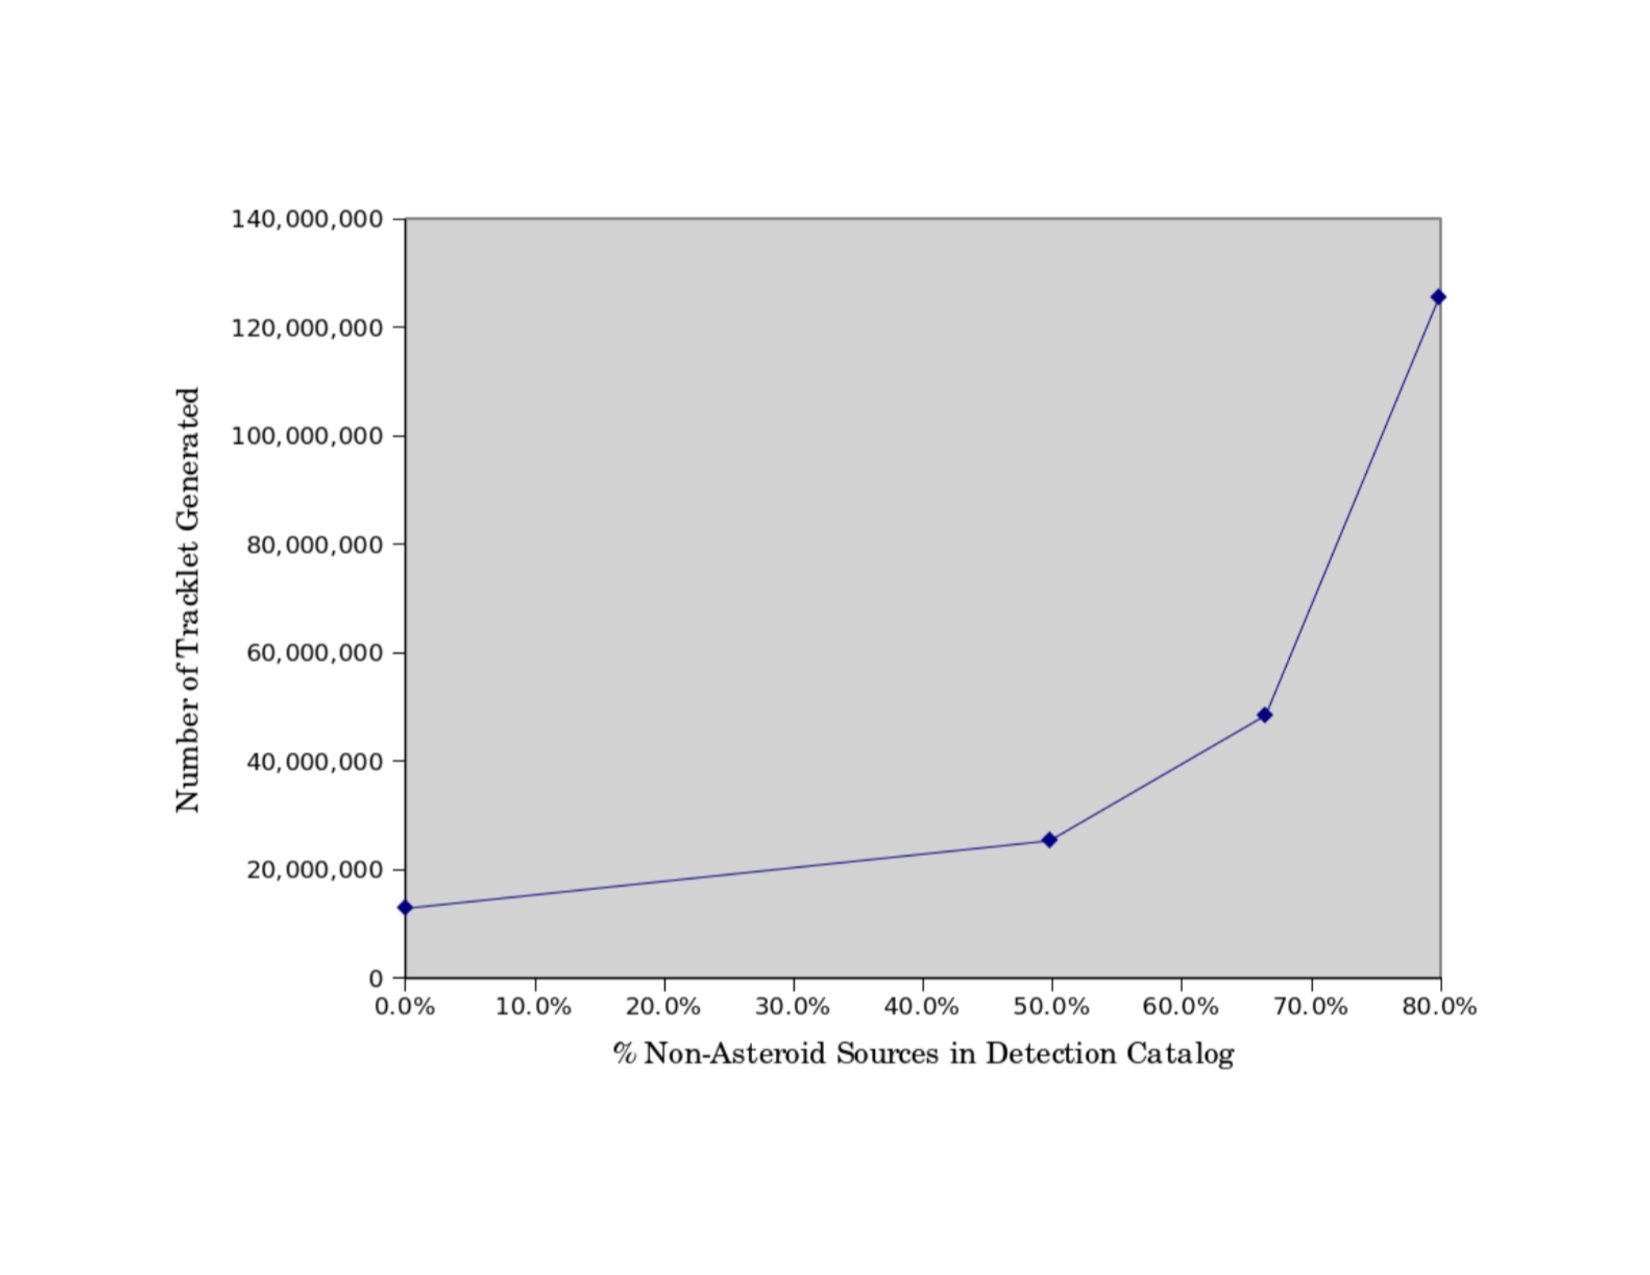
\includegraphics[width=0.49\textwidth]{figures/tracklet}
%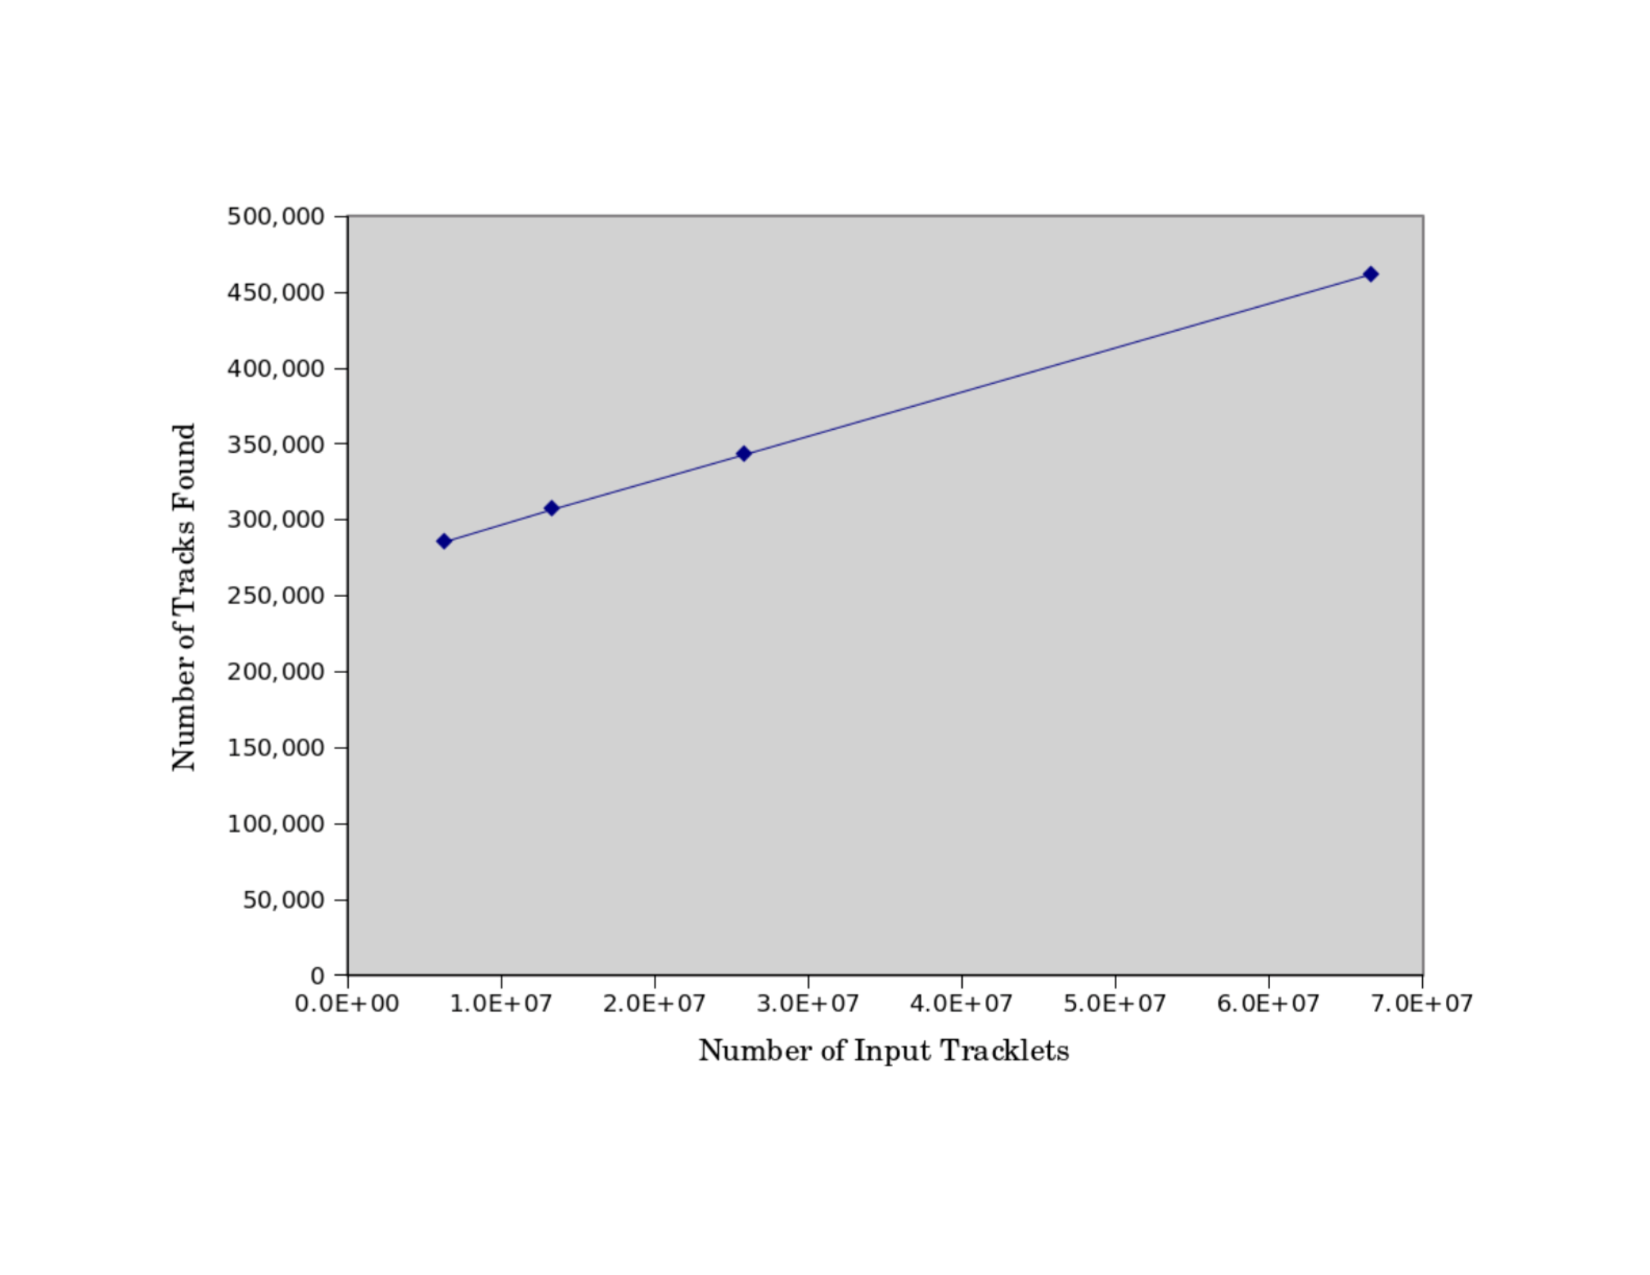
\includegraphics[width=0.49\textwidth]{figures/tracks}
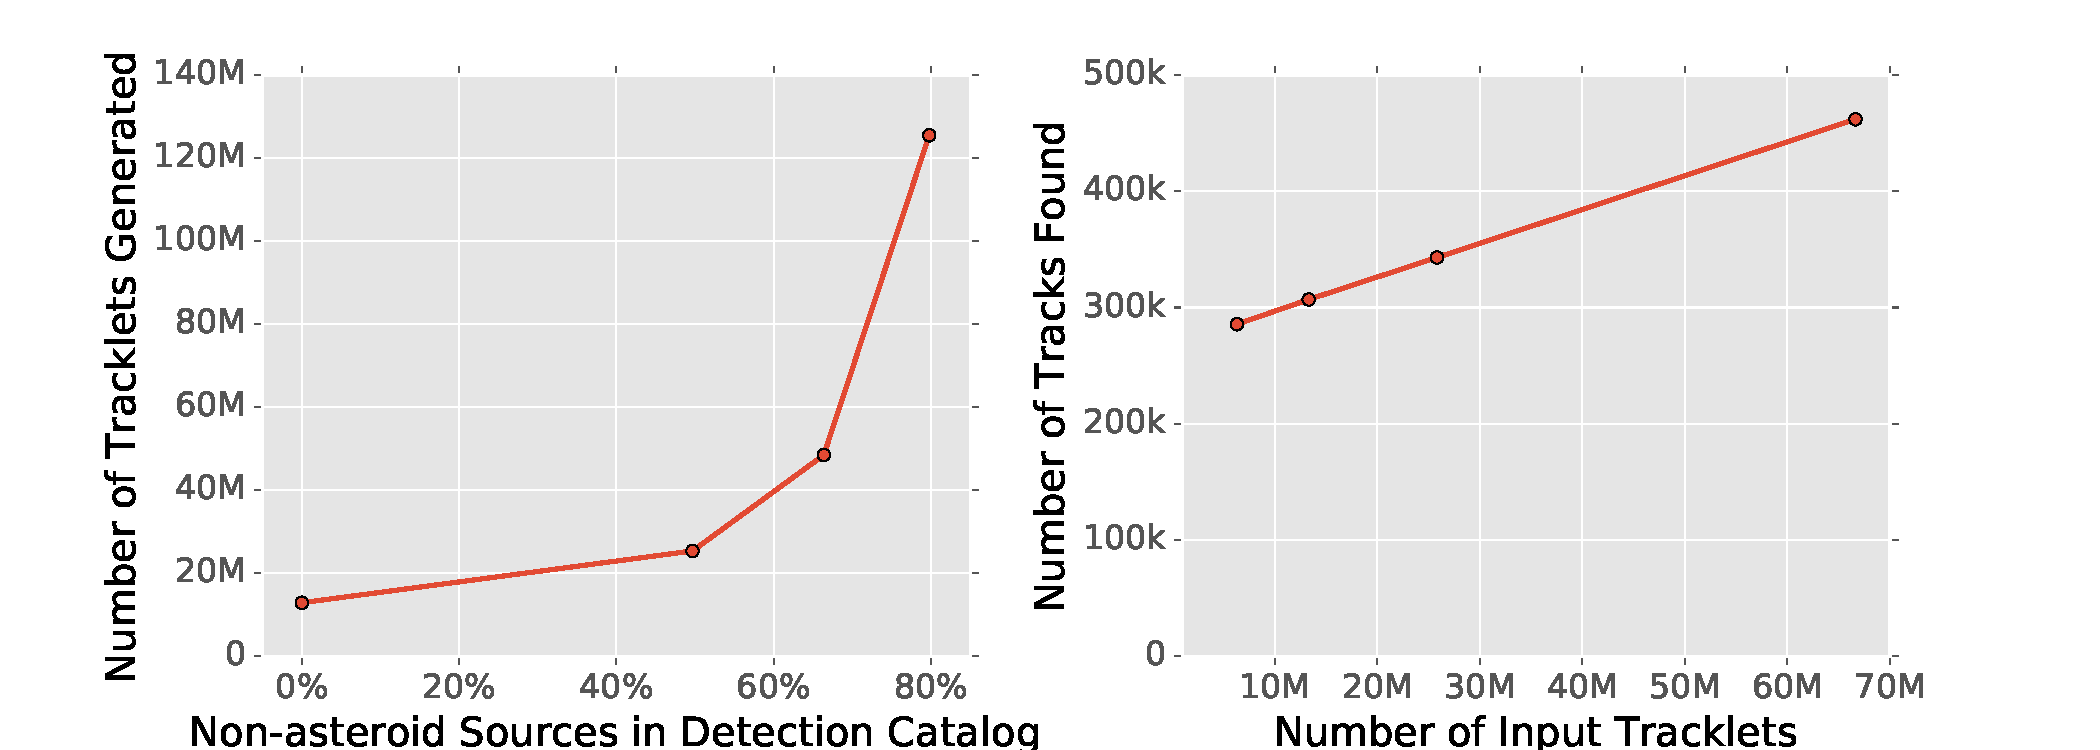
\includegraphics[width=0.95\textwidth]{figures/track_stats}
\caption{A summary of MOPS tests for the dependence of the number of tracklets (left)
and tracks (right) on the false positive detection rate. As the rate of false positive detections
increases from none to four times the asteroid detection rate, the number of tracklets
increases by about an order of magnitude. At the same time, the number of candidate
tracks increases by only about 50\%.
\label{fig:MOPStests}}
\end{figure}




\subsection{Understanding MOPS Performance}

The rather slow increase of the number of tracks with false positive detection rate (only 50\% increase
although the number of tracklets increased by a factor of 10) is somewhat unexpected. We have
developed analytic and semi-analytic analysis to better understand the scaling of the number of
tracklets and tracks with false positive detection rate and other relevant parameters. Details of this
analysis are provided in Appendix~\ref{sec:appMOPS}. Here we briefly discuss the main results.

The increase of the number of tracklets with false positive detection rate, $\rho_{FP}$, shown in left panel
in Figure~\ref{fig:MOPStests}, is well described by eq.~\ref{eq:NttFalse}. In particular, the number of tracklets
approximately increases proportionally to $(C_1 + C_2\rho_{FP}^2)$, where $C_1$ and $C_2$ do not
depend on $\rho_{FP}$. The reason why the ratio of the number of tracks and the number of tracklets
stays within a narrow 50\% margin when the latter varies by an order of magnitude (right panel
in Figure~\ref{fig:MOPStests}) is quantitatively explained by eq.~\ref{eq:NttFinalFit}.

The main result of our analysis is the scaling of the number of false candidate tracks per search window
with the window width and the density of false positives in difference images (for scalings with other relevant
parameters, see eq.~\ref{eq:falsetracks}),
\begin{equation}
\label{eq:falsetracks2}
   N^{falsetracks} = 4.5 \times 10^6 \, \left( {N_w \over 30 \, {\rm day} } \right)^{8} \left( {\rho_{FP} \over 400 \, {\rm deg}^{-2} }\right)^{3.7}.
\end{equation}
This expression is valid around fiducial values and assumes $\rho_{ast}=100$ deg$^{-2}$.
The number of true tracks is of the order 10$^6$; therefore, the false positive detections
in image differencing contribute only a factor of a few more candidate tracks for the IOD step.
Furthermore, even this small contribution could be decreased by decreasing the search window
width $N_w$ (at the expense of sample completeness). For example, for $N_w=21$ days,
the number of false tracks drops well below the number of true tracks.


\subsection{Required Computing Resources for MOPS and IOD Processing}

Given the modest computing resources used in MOPS tests described above, the runtime and memory
usage results bode well for LSST processing. Assuming a 1000-core machine dedicated to LSST moving
object processing (corresponding to about 1\% of the anticipated total LSST compute power at the
National Center for Supercomputing Applications, XXX check this with K.T.), MOPS runtime for
producing candidate tracks should not exceed an hour.

The IOD step can also be handled with anticipated resources. The number of available IOD computations
for a system a compute system with $N_{core}$ cores and allocated runtime $T_{runtime}$ can be estimated
as
\begin{equation}
  N_{IOD} = 3.6\times10^8 \left({ 0.1\,{\rm sec} \over T_{IOD}}\right) \,
                                         \left({ T_{runtime}  \over 10\,{\rm hr} }\right) \,
                                         \left({ N_{core}  \over 1000}\right).
\end{equation}
where $T_{IOD}$ is the time it takes to perform one IOD computation on a single core. Estimates
of $T_{IOD}$ are in the range 5--50 mas (50 mas is priv. comm. from Steve Chesley, and 5 mas is
from ``Pan-STARRS'', XXX we should have a better reference or rephrase), well below the fiducial
value of 100 mas adopted here. Given that the expected number of candidate tracks to filter using
IOD is well below $10^7$, it should be possible to accomplish the IOD step in well under an hour.
Alternatively, it is plausible that a 100-core machine might be sufficient for LSST moving object
processing (assuming no engineering safety margin).


\section{LSST Observing Cadence Optimization to Enhance PHA Completeness \label{sec:opsim}}

By observing in pairs of visits -- a strategy validated in the previous sections -- rather than triplets or quads of visits in each night, we can increase sky coverage and improve the survey efficiency. However, even within this constraint, there are multiple approaches to surveying the sky. In this section we will evaluate the effects of varying the LSST observing strategy and the resulting PHA completeness.

This evaluation will be carried out using a combination of the LSST Operations Simulator (OpSim) and the LSST Metrics Analysis Framework (MAF).
OpSim was previously described in section \ref{sec:strategy}. 
The LSST Metrics Analysis Framework (MAF) is a user-oriented, python package for evaluating the pointing history
from these simulated surveys in light of particular science goals or interests. The various metrics coded in the
MAF framework can be calculated for any given simulated survey and compared as proposal parameters are changed
in OpSim. This permits a thorough investigation of the trades between different observing strategies, in terms of the
effect on multiple science goals, including the PHA completeness.  We first describe the basic steps in our simulations,
then describe the baseline and modified LSST simulated surveys, and then discuss our results.


\subsection{Simulations of LSST Asteroid Discoveries}

The basic components of our end-to-end simulation of asteroid discovery, described in detail below, include
\begin{enumerate}
\item {\it NEO Population Modeling.} Orbital parameters are used to generate asteroid positions during the
simulated survey duration for a simulated or properly debiased extant NEO population. The population needs
to adequately sample color, size and other properties. A database of such positions evaluated with an adequate
time step  is available as an input to MAF.
\item {\it Survey Cadence Modeling.} A series of LSST pointings with instrumental metadata and observing conditions
is generated by OpSim. In addition to boresight positions, the camera orientation and selected filter, available
metadata enable the computation of instrumental sensitivity (limiting magnitudes).
\item {\it Asteroid Optical Flux Modeling.}  Optical flux from an arbitrary asteroid needs to be computed
as a function of the positions of the Sun, the asteroid and Earth, and asteroid physical properties (e.g., size
and color). This model is implemented in MAF. 
\item {\it Source Detection Modeling.} Given the instrument model, observing conditions and asteroid flux,
the signal-to-noise ratio is estimated and used to compute detection probability. This model is implemented
in MAF.
\item {\it Detection Linking Modeling.}  Instead of running MOPS, a model that emulates MOPS
performance is used to significantly speed up the computations. This model is implemented
in MAF.
\item {\it Completeness Estimation.} Given a list of ``discovered objects'', and the input population,
the completeness is estimated as a function of asteroid properties (e.g. size) and various other parameters
(e.g. observing strategy). This model is implemented in MAF.
\end{enumerate}

We proceed to describe these models in more detail, and then discuss the baseline and several modified LSST
surveys, and the corresponding PHA completeness estimates.

\subsubsection{NEO Population Modeling \label{sec:MAFdetails}}

We use random samples from the synthetic solar system model presented in \cite{Grav2011} in order to model completeness for NEOs and PHAs. We have chosen a sample of 2000 NEOs from the \cite{Grav2011} NEO population, which is based on the \cite{Bottke2002} model. We chose a separate sample of 2000 PHAs from the same model, by choosing NEOs with a MOID $\le 0.05$~AU. The PHA population is useful for evaluating PHA completeness directly; the NEO population is useful for comparison to other survey evaluations. A plot of the $a$, $e$, $i$ distributions for these PHAs and NEOs is shown in Figure~\ref{fig:PHA_orbits}.

With this small set of orbits, we then assume that the $H$ magnitude distribution is independent of the orbital distribution. For most small body populations, including the PHA population larger than 140~m in diameter, this is approximately true. Assuming an independent distribution, each orbit can be ``cloned'' from the fiducial $H$ magnitude to a range of values covering the interesting sizes for analysis; this allows the analysis to use a large number of objects at each $H$ value, without requiring extensive resources to generate ephemerides for a much larger set of orbits. We use the small population of 2000 NEOs or PHAs and clone them to a range of $H$ magnitudes between $H$=11 and $H$=28 using $dN/dH = 10^{\alpha\, H}$, with $\alpha=0.3$. We have verified with a larger simulated set of NEOs that reducing the population from 10,000 to 2000 objects does not change the calculated survey completeness significantly.

Using the details of the input population, MAF generates the expected observations of each object using the pointing history
from a specific OpSim simulated survey. Ephemerides are generated using OpenOrb \citep{OpenOrb2009} for a closely spaced grid
of times (typically every 2 hours), and then interpolated to the exact times of each OpSim pointing.


\begin{figure}[t!]
\centering
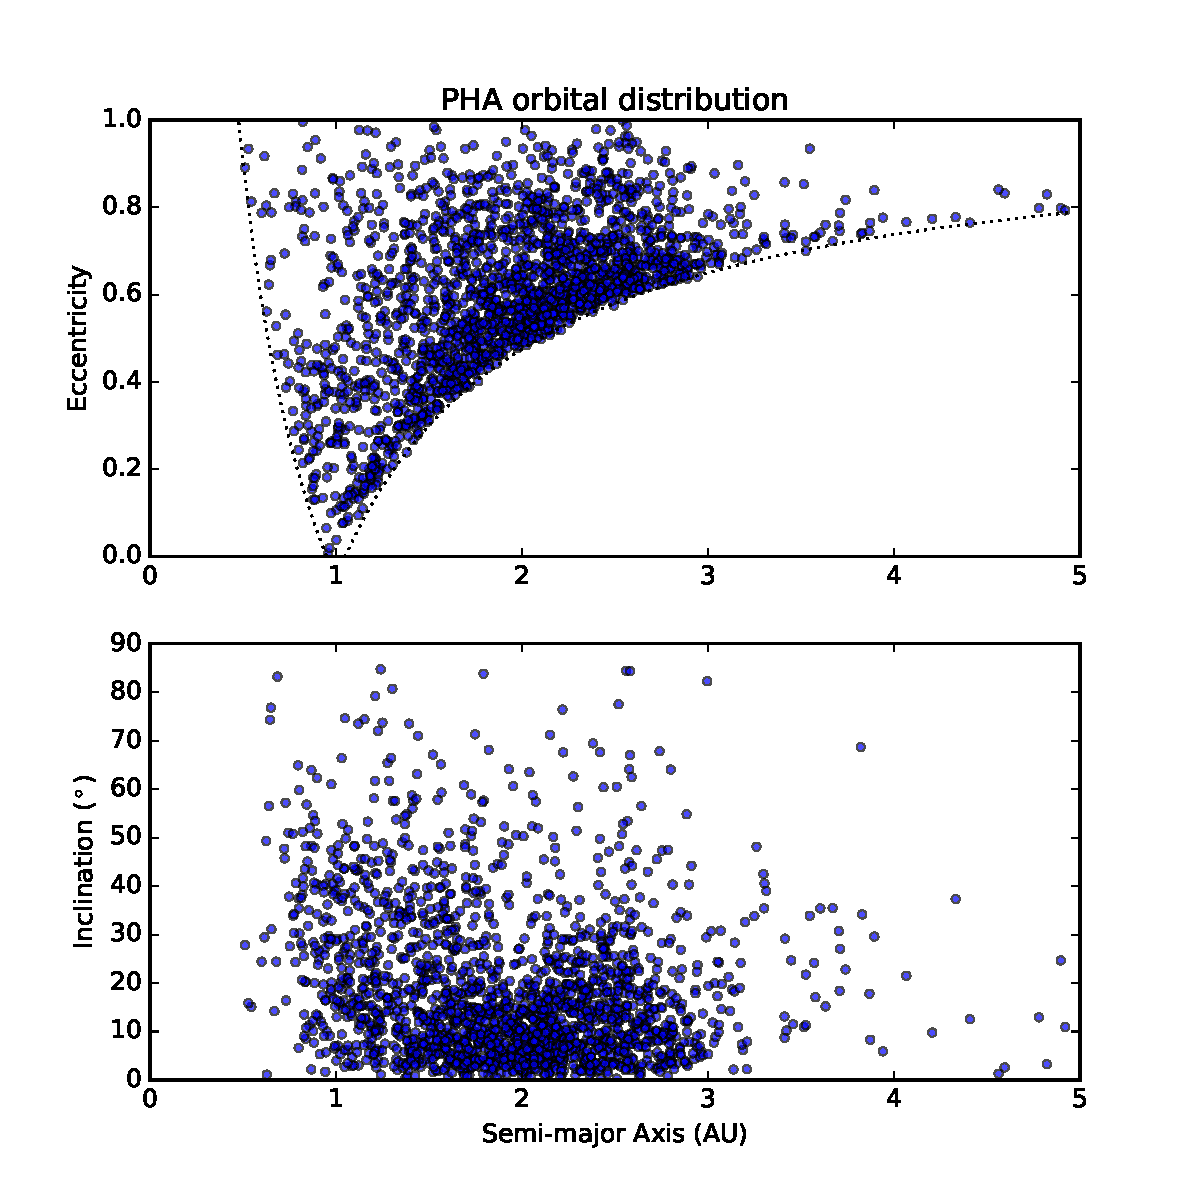
\includegraphics[width=0.49\textwidth]{figures/phas_2k_orbits}
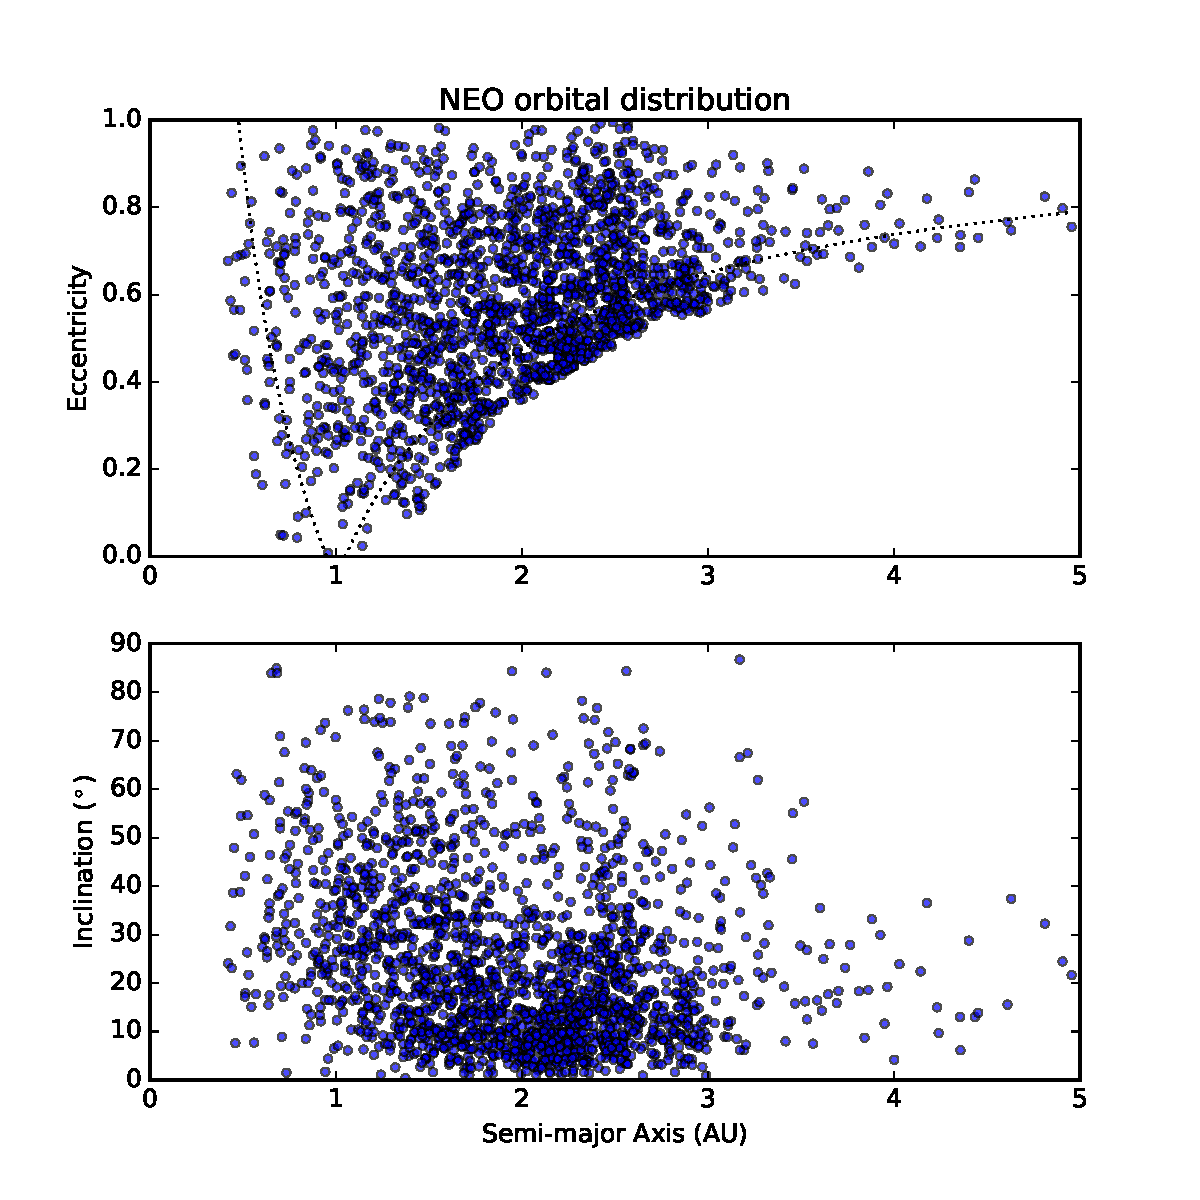
\includegraphics[width=0.49\textwidth]{figures/neos_2k_orbits}
\vskip -0.2in
\caption{The eccentricity and inclination distributions, as a function of semi-major axis, of the PHAs (left) and NEOs (right) used in this analysis. Both populations were randomly sampled from the S3M model \citep{Grav2011}, a synthetic solar system model based on the \cite{Bottke2002} NEO orbital distribution. NEOs are defined as objects with $q<1.3$~AU; PHAs are defined as having a Minimum Orbit Intersection Distance (MOID) with the Earth of less than 0.05~AU (implying $q\le1.05$~AU) and having $H\le22$.  \label{fig:PHA_orbits}}
\end{figure}

\subsubsection{Survey Cadence Modeling}

The LSST Operations Simulation \citep[OpSim,][]{delgado14} is a python software package that generates a realistic pointing history, with the time, filter, location, astronomical conditions, weather conditions, and predicted point-source $5\sigma$ limiting magnitude, for each LSST visit
for, typically, ten years. This pointing history is generated using weather data (cloudiness and seeing) from the Cerro Pachon site and a high-fidelity model of the telescope itself (including slew and settle time and dome movement, for example), combined with a parameterized set of observing proposals that determine how the scheduling algorithm attempts to gather observations. By configuring OpSim with different parameters for the observing proposals, we can generate a series of simulated surveys which prioritize different science goals. The LSST baseline survey and its modifications designed to enhance the PHA completeness are described in detail
in \S\ref{sec:surveys} below.


\subsubsection{Asteroid Optical Flux Modeling}

Given $H$ magnitude for an object, its apparent magnitude in Johnson's $V$ band can be easily computed
given the positions of the object, the Sun and the observer (e.g. \citealt{juric02}).
Magnitudes, or fluxes, in any other optical and near-IR band (in case of LSST, $u$, $g$, $r$, $i$, $z$, and $y$)
can be computed from $V$ magnitude by specifying a spectrum or relevant colors for each object. We have
assumed that our entire PHA population has the same colors as C-type main-belt asteroids, with resulting
transformations to  LSST bandpasses listed in Table~\ref{tab:sed_colors}. Choosing the colors of  S-type
main-belt asteroids instead results in $<$1\% changes in completeness.

\begin{deluxetable}{ccccccc}
\centering
\tablecolumns{7}
\tablecaption{Color transformations from Johnson's $V$ band to LSST bandpasses, for C and S type asteroids. \label{tab:sed_colors}}
\tablewidth{0.7\textwidth}
\tablehead{ Type & $V-u$ & $V-g$ & $V-r$ & $V-i$ & $V-z$ & $V-y$  \\ }
\startdata
C  & -1.53 &  -0.28 &  0.18 &  0.29 &  0.30 & 0.30 \\
S & -1.82 &  -0.37 &  0.26 & 0.46 &  0.40 & 0.41  \\
\enddata
\end{deluxetable}


\subsubsection{Source Detection Modeling}


\begin{figure}[t!]
\centering
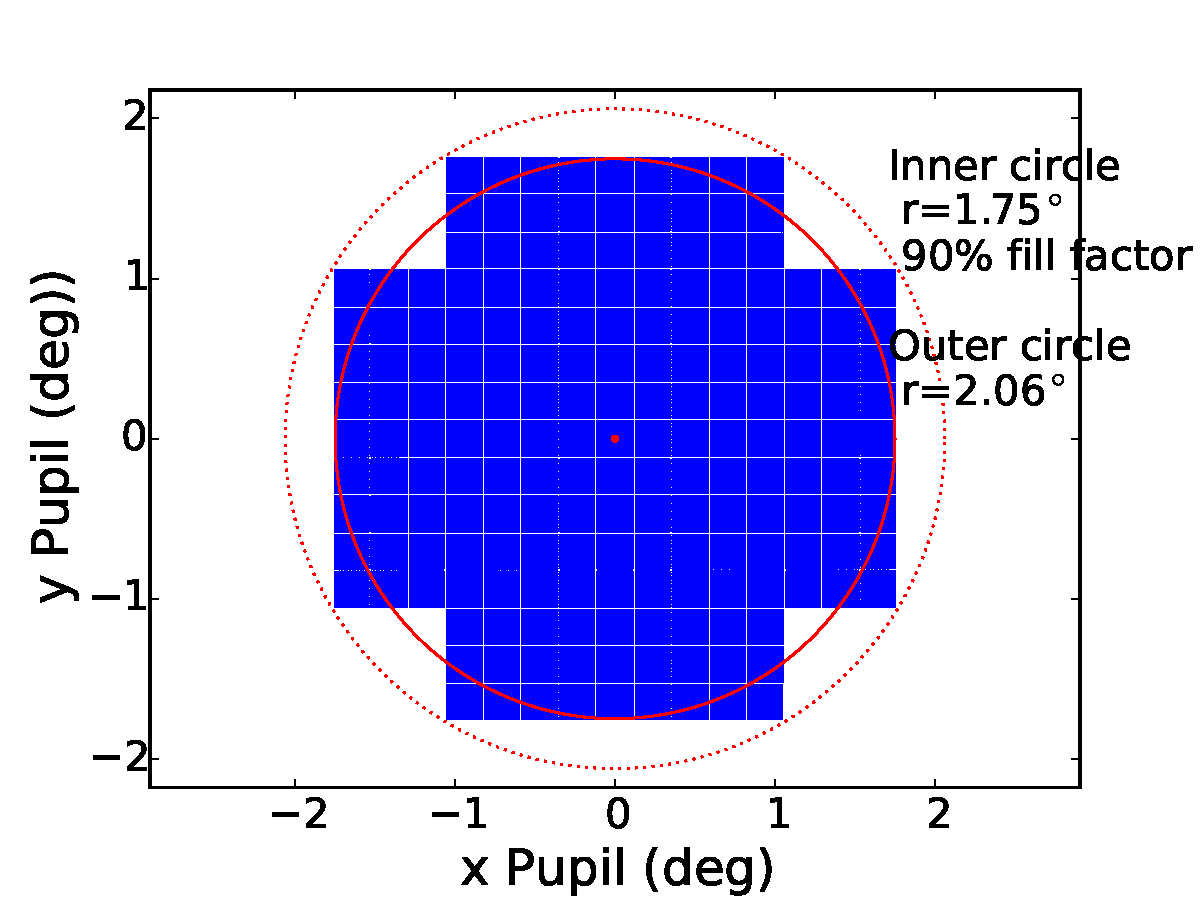
\includegraphics[width=0.65\textwidth]{figures/focalplane}
\caption{Model of the LSST camera footprint, including chipgaps and CCD + raft layout. \label{fig:camera_footprint}}
\end{figure}

If the object is within the LSST field of view, its predicted position, velocity, and apparent $V$ magnitude (calculated from the fiducial $H$ magnitude associated with the orbit) is recorded along with information about the simulated observation itself (such as the seeing, limiting magnitude, filter, and boresight RA/Dec). The full LSST camera footprint, including chipgaps, is used to determine whether
an object is within the field of view. The LSST camera footprint is shown in Figure~\ref{fig:camera_footprint}.

MAF also calculates trailing loss estimates for each observation, which are necessary when evaluating if a particular object is visible in a given observation. Trailing losses occur whenever the movement of an object spreads its photons over a wider area than a simple stellar point spread function (PSF). There are two aspects of trailing loss to consider: SNR losses and detection algorithm losses. The first is the
irreversible degradation in SNR that occurs because the trailed object includes a larger number of background pixels in its footprint, compared to a stationary PSF. The second effect, detection loss, occurs because source detection software is optimized for detecting point sources; a stellar PSF-like matched filter is used when identifying sources that pass above the defined threshhold. This filter is non-optimal for trailed objects but losses can be mitigated with improved software ({\it e.g.} detecting to a lower PSF-based SNR threshhold and then using a variety of trailed PSF filters to detect sources). When considering whether a source would be detected at a given SNR using typical source detection software, the sum of SNR trailing and detection losses should be used. With an improved
algorithm optimized for trailed sources (and this with additional workload on data management), the smaller SNR losses should be
used instead.

\begin{figure}[t!]
\centering
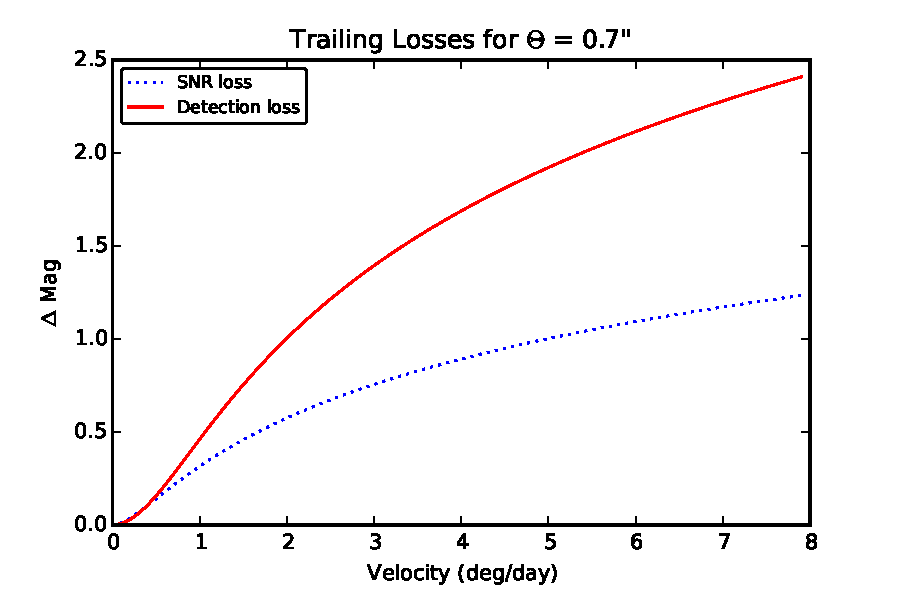
\includegraphics[width=0.85\textwidth]{figures/trailing_losses}
\caption{Trailing losses for 30 second LSST visits, assuming seeing of
  0.7''. The dotted line shows SNR trailing losses, the solid line
  indicates cumulative losses that also account for non-optimal detection
  algorithm. With software improvements the latter detection losses can be
  mitigated. At the fiducial $v=1$ deg/day, the SNR loss is $\sim$0.3 mag,
  and non-optimal detection algorithm contributes an additional loss of
  $\sim$0.16 mag.
\label{fig:trailinglosses}}
\end{figure}

Our simulations of these effects show that both trailing losses can be fit well with the
same functional form:
\begin{eqnarray}
\Delta \, m & = &-1.25 \, log_{10} \left( 1 + \frac{a \, x^2} { 1 + b\,
    x} \right) \\
x & = & \frac{v \, T_{exp}} {24 \, \theta}
\end{eqnarray}
where $v$ is the velocity (in deg/day), $T_{exp}$ is the exposure time (in seconds), and $\theta$ is the FWHM (in arcseconds). For trailing SNR losses, we find $a = 0.67$ and $b = 1.16$; for the cumulative loss, that includes both SNR and detection losses,
we find $a=0.42$ and $b=0$. An illustration of the magnitude of these trailing loss effects for 0.7 arcsec seeing is given in Figure~\ref{fig:trailinglosses}.

We calculate the probability of detecting a particular source given its magnitude $m$ (after accounting for trailing losses)
and the $5\sigma$ limiting magnitude $m_5$ using a logistic function
\begin{eqnarray}
     P & = & \left[ 1 +  {\rm exp}\left(\frac {m -  m_5}{\sigma}\right) \right]^{-1}.
\end{eqnarray}
where $\sigma$=0.12 describes the width of the completeness falloff \citep{2014ApJ...794..120A}. A source is randomly classified
as detected using the probability $P$. We also evaluate more optimistic discovery criteria using only SNR trailing losses
(i.e. without taking detection losses into account), as well as detections to SNR=4 instead of SNR=5.


\subsubsection{Detection Linking Modeling}

Given the set of visits where the object was within the field of view and detected, we look for visits spaced in time
according to the discovery criteria. These criteria generally consist of a given number of visits within a specified
time span within a single night, followed by a given number of additional nights (each with the same required number
of visits in the same time span) falling within a specified time window. The basic criteria is a pair of visits in each
night occurring within 60 minutes, repeated for 3 nights within a 15 day time window. However, we also evaluate
the effect of varying the discovery criteria to require triplets or quads of visits within a single night, and increase
the length of the search window from 15 to 30 days.


\subsubsection{Completeness Estimation}

With each unique set of discovery criteria, we have a record of what objects would be ``discovered'' at each $H$ value.
With this we calculate the differential discovery completeness, the fraction of objects discovered at a given $H$ magnitude.
To turn this into a cumulative discovery completeness, we simply integrate over $H$, assuming a given $H$ distribution
for the population (recall that we use $dN/dH = 10^{\alpha\, H}$, with $\alpha$ = 0.3).


\subsection{OpSim Simulated Surveys \label{sec:surveys}}

\subsubsection{The LSST Baseline Survey}

The current baseline observing strategy for LSST is represented by our reference run, minion\_1016. This simulated survey
contains observations balanced between several different observing proposals:
\begin{enumerate}
\item The Wide, Fast, Deep (WFD) proposal (also known as the Universal proposal) is the primary LSST survey, expected to receive about 90\% of the observing time and to cover 18,000 deg$^2$ of sky. In the baseline observing strategy, this proposal is configured to obtain visits in pairs spaced about 30 minutes apart, and will typically return to each field about every 3-4 days, balancing the six $ugrizy$ filters. The footprint for the WFD proposal covers approximately $+5^\circ$ to $-60^\circ$ in declination, with a full range of RA values except for a region around the Galactic plane. This declination range corresponds to an airmass limit of about 1.3 when the fields are at an Hour Angle of $\pm$2 hours. In minion\_1016, the WFD proposal receives 85\% (2,083,758) of the total number of visits.
\item The North Ecliptic Spur (NES) proposal is an extension to the WFD to reach the northern limits of the Ecliptic plane ($+$10 degrees), and allows higher airmass observations. The visit timing is similar to the WFD, although the $u$ and $y$ filter are not requested in this region. In the baseline observing strategy, minion\_1016, each NES field requests about 40\% of the total number of WFD visits per field when considering $griz$ filters only (304 visits per field in $griz$ vs 795 visits per field in $griz$ in WFD), and receives 6\% (158,912) of the total number of visits.
\item The Deep Drilling Fields (DD) proposal includes a set of single pointings that are requested in extended sequences; currently these sequences are $grizy$ visits, with additional coverage in $u$ band. Each sequence requires about an hour of observing time, and is repeated every few days. In minion\_1016, there are 5 DD fields, 4 of which correspond to fields which have been officially selected
by the Project and announced to the community; these five fields receive 5\% of the total visits.
\item The Galactic Plane (GP) proposal covers the region with high stellar density around the Galactic plane not covered by the WFD. This proposal requests a small number of visits in each of the six $ugrizy$ filters, with no timing constraints. In minion\_1016, this proposal receives 2\% of the total visits.
\item The South Celestial Pole (SCP) proposal is an extension of the WFD footprint to cover the region south of $-60^\circ$ declination. Like the GP, this proposal requests a small number of visits in each of the six $ugrizy$ filters, with no timing constraints. In minion\_1016, this proposal receives 2\% of the total visits.
\end{enumerate}

The footprint of these various proposals in the baseline minion\_1016 reference run is shown in Figure~\ref{fig:minion_footprints}. In each proposal, the individual visits are 30 seconds long, consisting of two back-to-back coadded 15 second exposures.

\begin{figure}[t!]
\centering
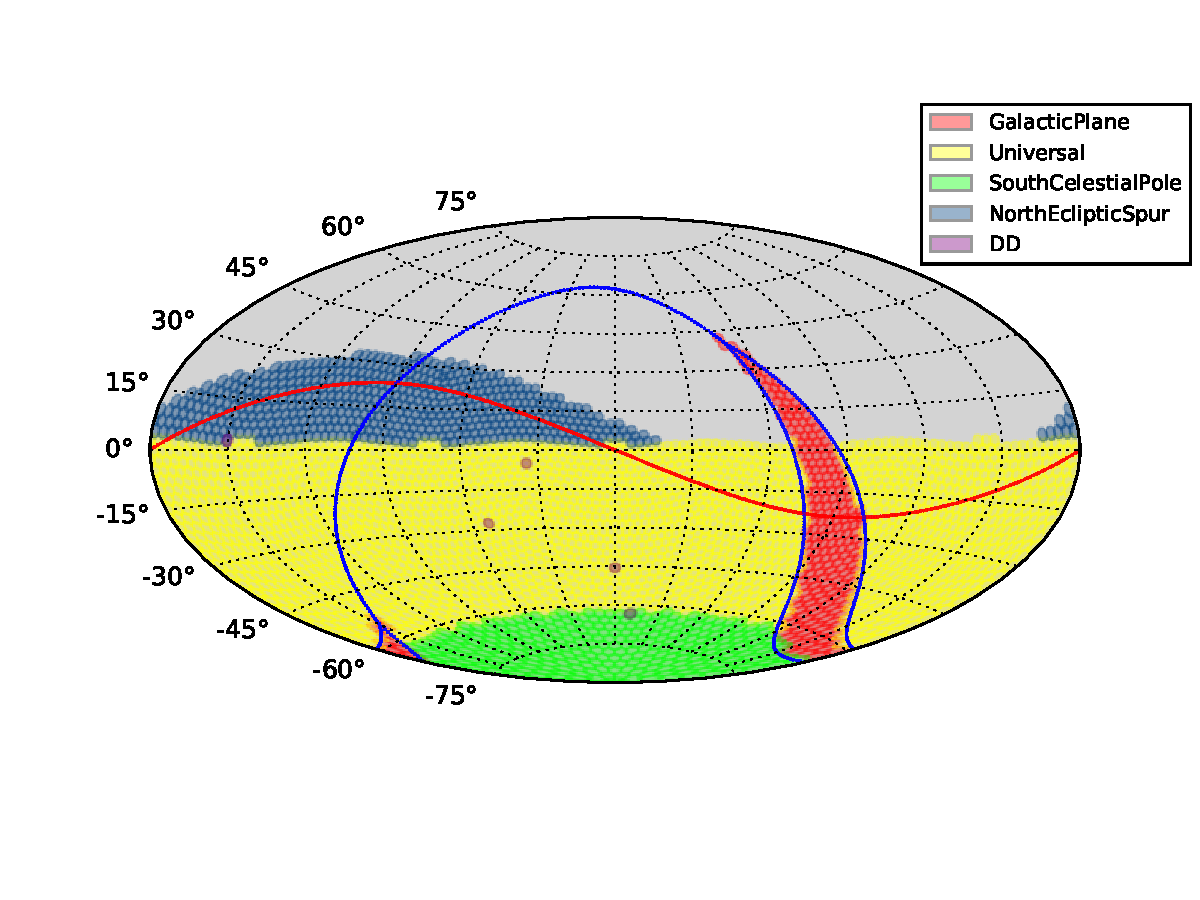
\includegraphics[width=0.85\textwidth]{figures/minion_1016_proposal_footprint}
\vskip -1.0in
\caption{The footprints of the various proposals included in the baseline observing strategy, represented by reference run minion\_1016.
\label{fig:minion_footprints}}
\end{figure}


\subsubsection{Modified Surveys}

A series of additional OpSim simulated surveys were created with parameters intended to improve the efficiency of discovering PHAs and increase the cumulative PHA completeness. They span the range from minor modifications to extreme changes that would
jeopardize other LSST science goals. We consider the latter in order to assess what would be ultimate performance of an
LSST-like system fully dedicated to NEO surveying.

\textbf{Extra ecliptic spur visits:} The first cadence change is simply to increase the number of visits requested for the NES proposal in $griz$, to increase the likelihood of discovering objects near the northern portion of the Ecliptic plane, and to extend the survey from 10 years to 15 years, increasing the discovery rate of PHAs with long synodic periods. Other proposals remain the same as in minion\_1016. Reprioritizing the NES relative to the WFD results in the WFD receiving 69\% (2,561,334 visits over 15 years) of the total visits and the NES receiving 24\%, compared to 85\% and 6\% respectively in the baseline strategy. The resulting simulated survey is astro\_lsst\_01\_1016.  We consider astro\_lsst\_01\_1016 as our 'baseline PHA' run, as it makes minimal changes to the overall survey strategy while attempting to be more PHA friendly.

\textbf{Longer ecliptic visits:} This simulation introduce an Ecliptic Band (EB) proposal, requesting observations with visit timing similar to the WFD in the $griz$ filters, but with field locations surrounding the Ecliptic Plane $\pm15^\circ$ and extending down to the WFD where the Ecliptic reaches its northernmost  range. This proposal replaces the NES proposal, and requests longer 60 second visits in order to reach deeper limiting magnitudes. Other proposals remain the same as in astro\_lsst\_01\_1016. With this reprioritization, the WFD receives 44\% (1,159,319) of the total visits while the EB receives 53\%; the simulated survey is astro\_lsst\_01\_1015.

\textbf{NEO-focused survey:} An attempt at an aggressively NEO-optimized survey was also created, where modified versions of the EB and WFD proposals are used. The visit timing in each proposal is the same as the standard WFD visit timing (a pair of visits separated by about 30 minutes), however the WFD footprint is changed to simply cover the entire area between 0$^\circ$ and $-60^\circ$ declination except for the EB footprint. The EB and WFD proposals request observations in only $gri$ filters, with 30 second visits in the WFD and 60 second visits in the EB. No other proposals are included. The resulting simulated survey is astro\_lsst\_01\_1017.

\begin{figure}[t!]
\centering
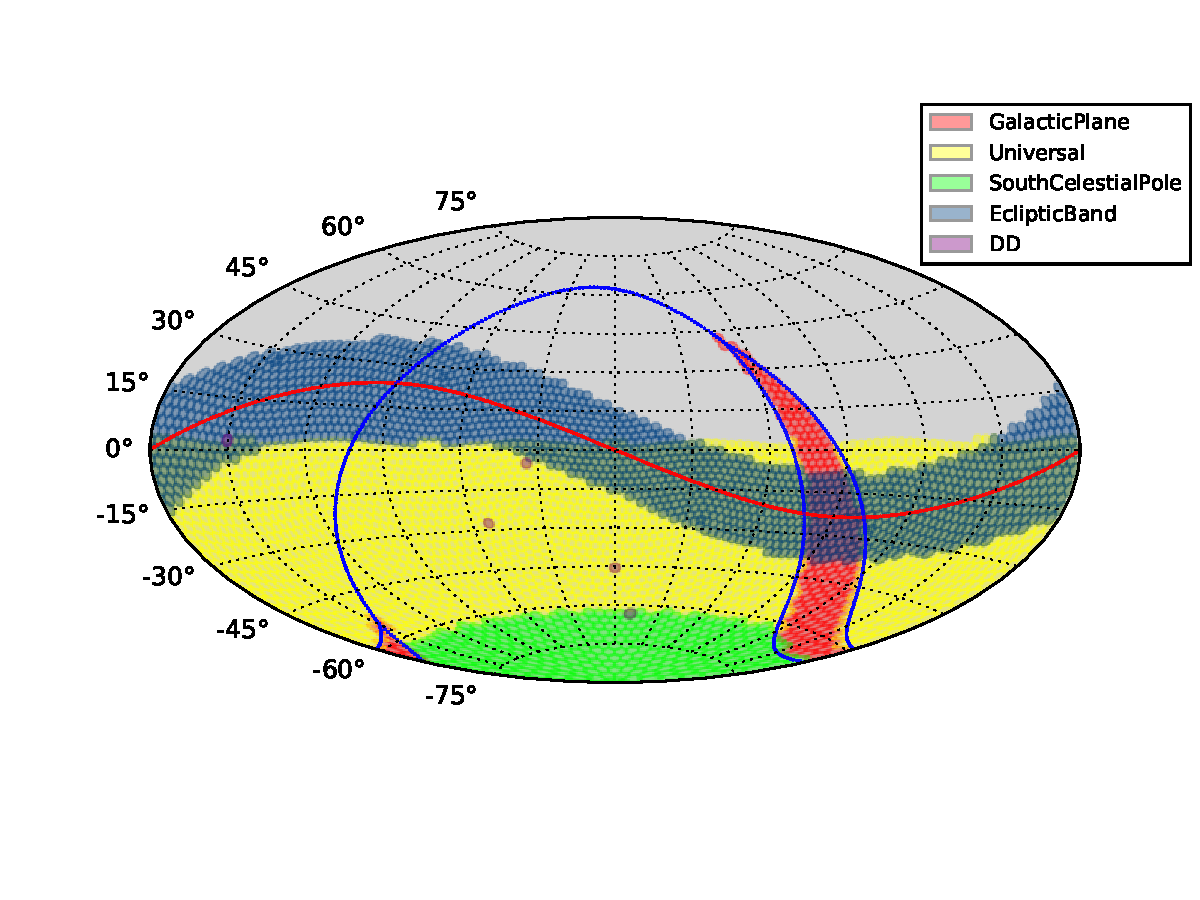
\includegraphics[width=0.49\textwidth]{figures/astro_lsst_01_1015_proposal_footprint}
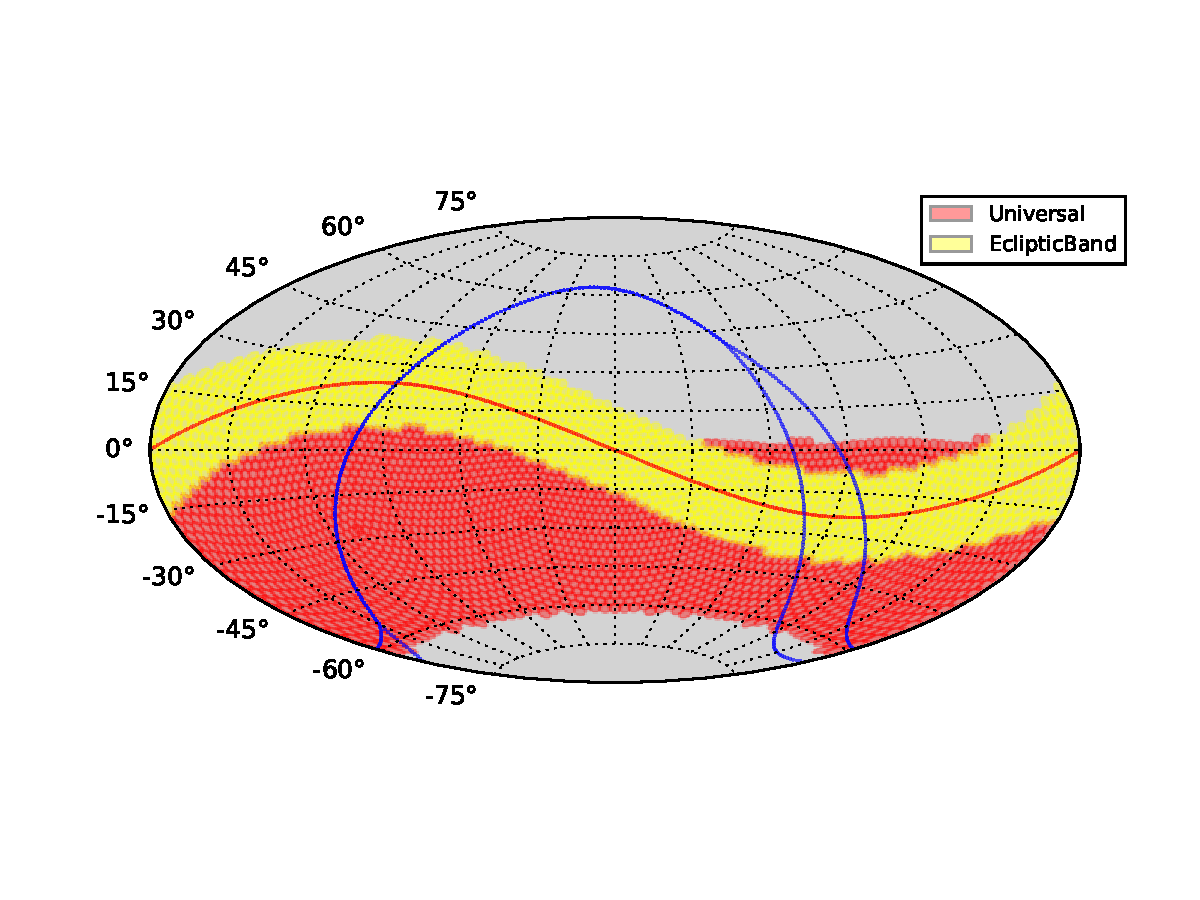
\includegraphics[width=0.49\textwidth]{figures/astro_lsst_01_1017_proposal_footprint}
\vskip -0.5in
\caption{The footprints of the proposals, including the Ecliptic Band proposal, used in the NEO-optimized simulated surveys astro\_lsst\_01\_1015 (the ``longer ecliptic visits'' survey, left) and astro\_lsst\_01\_1017 (the ``NEO-focused'' survey, right). The astro\_lsst\_01\_1017 survey only includes two proposals.
\label{fig:neo_footprints}}
\end{figure}


\subsection{Completeness analysis results}

In the baseline reference run, minion\_1016, with the baseline discovery
criteria, with pairs of visits in each night occurring within 60 minutes
repeated for 3 nights within a 15 day time window, we find a cumulative
completeness at $H\le22$ of 65.6\% for our PHA input population (see
Figure~\ref{fig:minionC1}). This should be considered our baseline PHA
completeness, as it uses the reference run and the baseline MOPS and data
management requirements.

From this baseline, we can evaluate the effects of changing both the survey design (reallocating telescope resources) and the discovery criteria, which effectively sets the computational resources.
There is an interplay between discovery criteria and survey design -- as an obvious example, discovery criteria requiring triplets of visits per night instead of pairs will result in much different completeness results if the survey was designed to only request two visits per night rather than three. Likewise, some changes in survey design work best with changes to the discovery criteria; for example, lengthening the visit time increases the detection losses, which means pushing source detection to the ``trailing loss'' threshold results in a significant improvement in completeness. While we compare discovery criteria within a single simulated survey as much as possible, there are some changes in discovery criteria which must be compared between different surveys using different observing strategies.

All the completeness results presented below assume that no objects are known prior to LSST survey,
and thus are biased low. For example, by assuming that 43\% PHAs would be discovered by the start of
LSST survey, \cite{GMS2016} showed that the final PHA completeness for LSST baseline survey would
be boosted by 11\%. We discuss our own independent estimates of this effect in \S\ref{sec:known}.

\begin{figure}[t!]
\centering
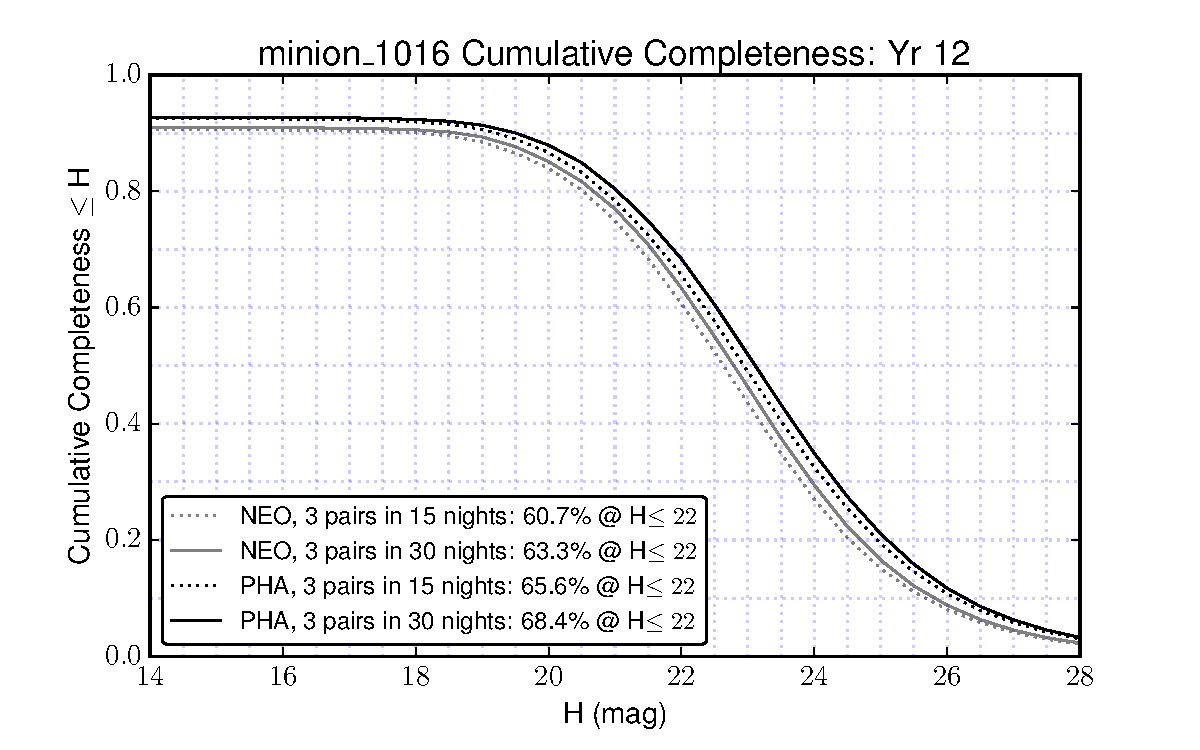
\includegraphics[width=0.99\textwidth]{figures/minion_1016_CumulativeCompleteness_NEO_and_PHA_Cumulative_Completeness}
\vskip -0.2in
\caption{The cumulative completeness for PHAs and NEOs, as a function of absolute magnitude $H$, for the baseline
cadence minion\_1016. \label{fig:minionC1}}
\end{figure}

\begin{deluxetable}{lccccccc}
\tablecaption{The cumulative completeness for PHAs with $H\le22$ for various
survey strategies (rows) and discovery criteria (columns). In addition to
changing the overall duration of the survey (12 years instead of 10), the
completeness is shown for different track linking windows (W=15 or 30 days),
enhanced detection algorithms to reduce trailing losses (``Trail Det''), and
pushing the individual detection threshold from SNR$=5$ to SNR$=4$. These are
primarily computational changes, while the various rows show different survey
cadences. These range from the current baseline, to adding additional visits or
longer visits in the ecliptic region, to focusing the majority of the time on
performing a NEO-focused survey. \label{tab:completeness}}
\tablehead{
& \multicolumn{3}{c}{10 year survey}  &  \multicolumn{4}{c}{12 year survey}  \\
\cmidrule(r){2-4} \cmidrule(r){5-8}
Simulation  & W=15 & W=30 & W=30 & W=15 & W=30 & W=30 & W=30 \\
            &      &      & Trail Det&  & & Trail Det & SNR=4 \\
%            &      &      &      &      & &           & SNR=4
}
\startdata
LSST baseline & 65.5 & 68.4 & 69.1 & & &  \\
Extra ecliptic visits & 66.1 & 69.8 & 70.5 & 70.5 & 73.9 & 74.8 & 77.1\\
Longer ecliptic visits & 63.2 & 67.5 & 70.5 & 67.3 & 71.7 & 74.5 & 75.7 \\
NEO-focused cadence & 66.5 & 70.3 & 72.3 & 70.2 & 73.8 & 75.8 & 77.2 \\
\enddata
\end{deluxetable}


\subsubsection{Modified Discovery Criteria \& Computational Strategies}

Using only the baseline minion\_1016 and not changing the survey strategy, we can explore the impact on PHA completeness of changing the discovery criteria. These are correspond primarily to the different columns of Table~\ref{tab:completeness}, and include:

\begin{itemize}
\item extending the MOPS window for linking pairs of detections from the nominal 15 day window to a 30 day window: this increases completeness by about 3\%, although with an estimated increase in the compute requirements by about an order of magnitude (see Appendix \ref{sec:appMOPS}).
\item enhancing source detection algorithms to mitigate detection losses to the trailing loss level: with the 30 second visits in the baseline minion\_1016, this only increases completeness by a very small amount, 0.5\%.
\item using sources detected down to SNR=4 instead of SNR=5: this increases completeness by about 2-3\%, although with an estimated increase in the compute requirements by about two orders of magnitude (see \S\ref{sec:kaiser}).
\end{itemize}

The major gain available in the baseline survey (or any survey with a maximum visit time of 30 seconds) is through increasing the MOPS linking window from 15 to 30 days. This allows more opportunities to capture the PHAs in a set of observations which meet the discovery criteria. It is worthwhile to note that the current OpSim behavior does not prioritize capturing large chunks of contiguous sky, and often leaves gaps in coverage from night to night. This behavior is likely related to the increase in completeness going from 15 day windows to 30 day windows; with the large LSST field of view, after 30 days the areal coverage will be much more evenly distributed than after 15 days. Changes to the scheduling algorithm to favor covering contiguous blocks of sky\footnote{A similar modification of
the baseline cadence, the so-called ``rolling cadence'', is also favored by the supernovae science programs. A release of a series of simulated surveys implementing this idea is anticipated for late 2017.} are likely to improve the completeness even further.  Pushing to SNR=4 exceeds the expected compute resources and is not worthwhile in comparison.


When an NEO population is used instead of a PHA input population, the cumulative completeness is between 6-10\% lower
(see Figure~\ref{fig:minionC1}). This is primarily due to differences in their orbital distributions, as illustrated in Figure~\ref{fig:PHA_orbits}. The definition of PHAs includes a Minimum Orbit Intersection Distance (MOID) with Earth of 0.05~AU, requiring PHAs to more closely approach Earth than NEOs (which are defined as simply having $q<1.3$~AU), and thus the PHAs achieve brighter peak V magnitudes than the NEOs. To quantify this effect, we calculated the apparent $V$ magnitude for both the NEO and PHA input populations every night for ten years, while accounting for trailing losses and assuming a constant $H=22$ magnitude for every member of the population. The resulting distributions of the
brightest 10-year $V$ magnitude values are shifted by about 0.03 magnitudes (the mean brightest magnitude values are 22.3 for NEOs and 22.6 for PHAs).


\subsubsection{The Performance of Modified Surveys}

The potential improvement in PHA discovery rates for modified survey cadences is
summarized in the rows of Table~\ref{tab:completeness} and described below.

\begin{itemize}
\item \textbf{Extra ecliptic spur visits:} By adding these extra visits over the course of a 10 year survey, the increase in completeness over the LSST baseline is about 1\%. This improvement comes at a cost to other science cases, as the main survey footprint (the WFD proposal) only receives 1,715,354 visits (82\%) of the number of visits in the reference run; the outcome of many science programs is roughly proportional to the number of visits.
\item \textbf{Extending the survey by two years:} Since minion\_1016 is a reference run, it only simulates 10 years.
However, we can evaluate the ``extra ecliptic visits'' run at the 12 year mark, at which point the WFD proposal has received approximately the same number of visits as it would receive in the baseline 10 year survey. The additional two years of operations adds just over 4\% to the completeness, going from 66.1\% at 10 years to 70.5\% at 12 years.
\item \textbf{Longer visits in the ecliptic:} This reaches fainter limiting magnitudes, but the effect of longer exposures alone is minimized by the fact that detection losses are also increased. It is also hard to disentangle the effects of increasing the visit time near the Ecliptic and the resulting lower frequency of observations (and thus fewer opportunities for sets of observations matching the basic discovery criteria). The small modifications made by this survey strategy show almost no change in completeness, {\it until} detection losses are partially compensated for by modifying source detection algorithms to the trailing loss level; then this run provides a 1\% increase in completeness compared to the ``extra ecliptic visits'' survey at twelve years.
\item \textbf{Aggressively NEO-focused survey:} This survey uses a limited filter set, discards other proposals, and uses longer exposures along the ecliptic. This survey shows an increase in completeness (75.8\%), relative to the ``extra ecliptic visits'' survey of about 1.5\%, after using longer MOPS windows and pushing source detection to the trailing loss level.
However, many science programs would be jeopardized with this observing strategy because observations in the $uzy$ filters,
and observations of the DD and SCP fields, would not be obtained.
\end{itemize}

To summarize, when altering the survey strategy the largest individual gain ($\sim$4\%)
comes from simply extending the survey lifetime from 10 to 12 years. For the case of PHAs and 30-day wide MOPS window,
the completeness can be boosted from 65.6\% after 10 years with minion\_1016 survey to 73.9\% after 12 years with
``extra ecliptic visits'' survey (recall that this completeness estimates do not account for the contribution of known objects).


\subsection{The Impact of Objects Known Prior to LSST Survey \label{sec:known}}

The completeness results presented above assumed that no objects are known prior to LSST survey.
By including known objects, the completeness is boosted to higher values; the current completeness
for NEOs with $H<22$ is estimated to be about 25\% \citep{GMS2016}. According to the JPL NEO
discovery page\footnote{See http://neo.jpl.nasa.gov/stats/}, one can conservatively estimate that
discovery of 140m NEOs started in earnest in 2000.

We use a simplified model to estimate the contribution of known objects: since we do not know the
survey pointing history for all the previous surveys, we simulate them by adopting an effective
Johnson $V$ magnitude threshold, $V_{max}$. We integrate orbits for our synthetic NEO model
population from 2000 to 2015 and consider an object discovered if its peak $V$ magnitude
during that period is brighter than $V_{max}$. We vary $V_{max}$ threshold until the completeness
for NEOs with $H<22$ in 2015 is $\sim$25\%. We obtained $V_{max}=20.0$ (this threshold
produces a completeness of 95\% for NEOs with $H<18$, i.e. for canonical objects larger than 1 km).
We continue ``discovering'' objects with $V_{max}=20.0$ until the beginning of LSST survey in 2022
(yielding 30\% completeness for NEOs with $H<22$, and 39\% for PHAs). All objects discovered prior
to 2022 that were {\it not} re-discovered by LSST are added to post-LSST sample. 
This likely underestimates the completeness boost added by other surveys, as it simply assumes the same discovery rate as seen over the past fifteen years, but does not include any improvements (in depth or sky coverage) in those other surveys.

Our results are summarized in Figure~\ref{fig:knownObj} and Table~\ref{tab:completeness2}.
For example, the completeness for PHAs is boosted by 7\% for baseline 10-year survey,
a somewhat more modest effect than 11\% boost obtained by \cite{GMS2016}. For a 12-year
survey, we predict a completeness of 80\% for PHAs, when known objects are taken into account.


\begin{deluxetable}{lcccc}
\tablecaption{The cumulative completeness (in \%) for NEOs and PHAs with $H\le22$ for
LSST baseline survey strategy extended to a 12-year survey (with some extra visits along the
Ecliptic, corresponding to the second row in Table~\ref{tab:completeness}). The length of track
linking window is set to 30 days, and the detection threshold is set to SNR$=5$.
\label{tab:completeness2}}
\tablehead{
& \multicolumn{2}{c}{10 year survey}  &  \multicolumn{2}{c}{12 year survey}  \\
\cmidrule(r){2-3} \cmidrule(r){4-5}
Population  & only LSST & w/ known &  only LSST & w/ known 
}
\startdata
    NEO    & 64 & 70 & 68 & 73  \\
    PHA    & 70 & 77 & 74 & 80  \\
\enddata
\end{deluxetable}


\begin{figure}[t!]
\centering
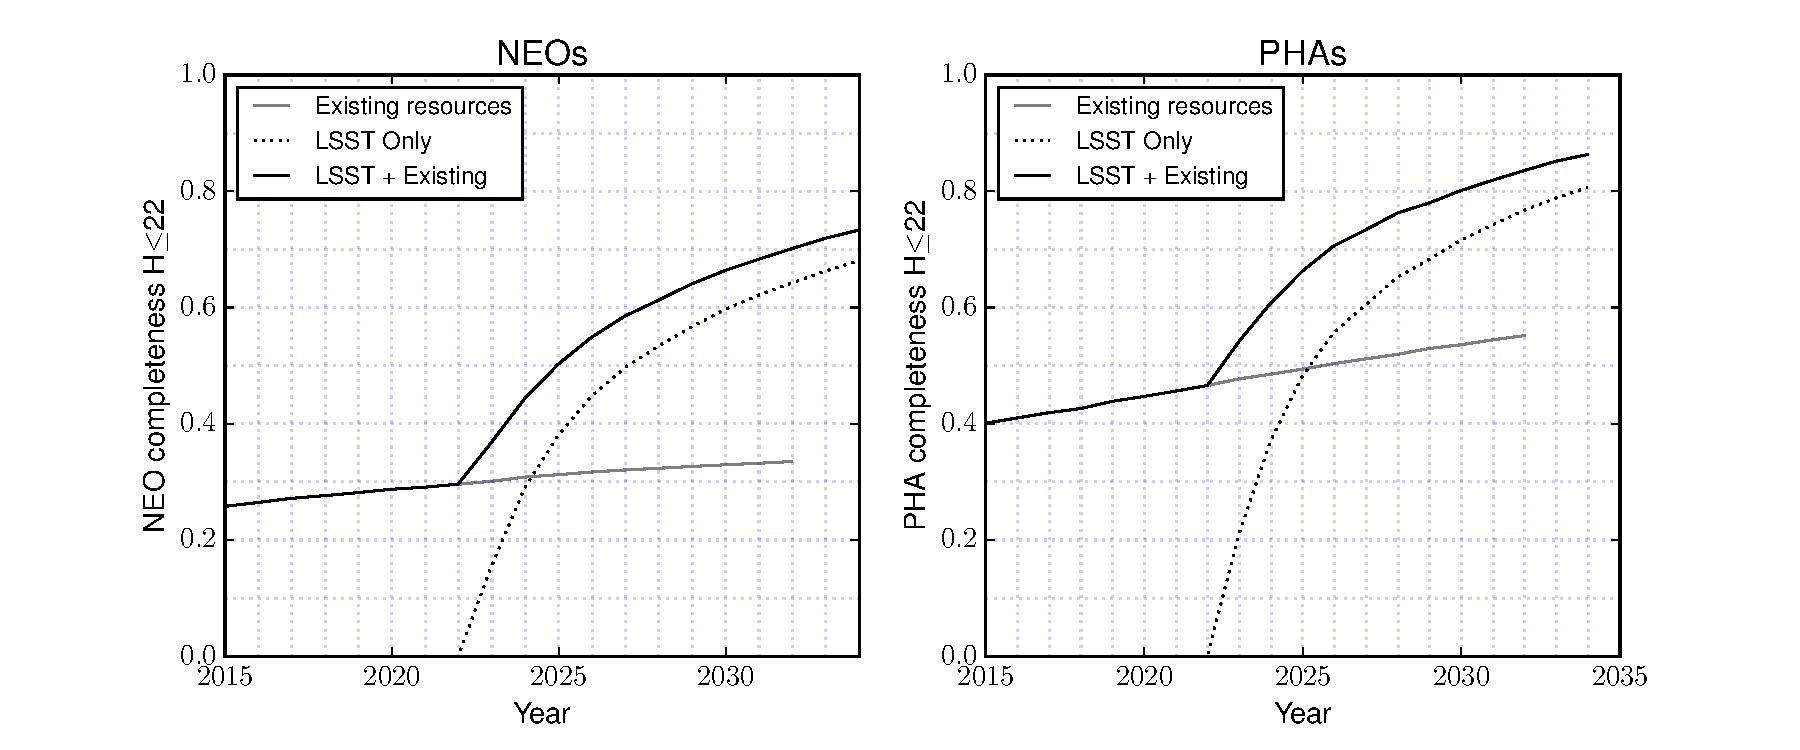
\includegraphics[width=0.99\textwidth]{figures/astro_lsst_01_1016_completeness.pdf}
\vskip -0.2in
\caption{The cumulative completeness for NEOs (left) and PHAs (right) with $H\le22$, as a function of
time, when known objects (gray solid lines) are taken (black solid lines) and not taken (dotted lines)
into  account (see also Table~\ref{tab:completeness2}).
\label{fig:knownObj}}
\end{figure}



\subsection{Systematic Effects due to Varying Modeling Assumptions \label{sec:syseff}}

As indicated by the above discussion, a number of systematic effects must be taken into account when
comparing different simulations of the same survey, as well as simulations of different surveys and observing
systems. It is unlikely that a meaningful quantitative comparison can be pushed beyond a level of a few percent
in completeness (in practice, the completeness of a given operating survey is best estimated using the object
re-discovery rate). Based on our analysis, the leading systematic effects in simulated completeness estimates are:
\begin{enumerate}
\item NEO vs. PHA difference. The completeness is about $\sim$6-10\% higher for PHAs than for NEOs;
for minion\_1016, the cumulative completeness is 65.6\% for PHAs and 60.7\% for NEOs.
\item Orbital parameter distribution for the simulated asteroid population (e.g. the Bottke model
             vs. the Granvik model); varying populations contribute completeness uncertainty of about a few percent)
\item Different sample definitions: $H<22$ vs. $D>140$m (as shown by \citealt{GMS2016}, completeness
           increases by $\sim$5\% when $H$-based criterion is used)
\item Variations of the ``discovery window'' (e.g., X visit pairs in N nights: changing N from 15 to 30 with X=3 increases
          completeness by about 3\%; changing X from 3 to 4 with N=15 decreases completeness by 6\%).
\item Uncertainties when predicting effective image depth (system throughput, variation of the detection efficiency
          with the signal-to-noise ratio, treatment of trailing losses); for a survey that has a completeness above 60\%,
          each additional {\it 0.1 magnitude of depth for a given survey cadence increases the completeness by another 1\%}.
\item Uncertainties when predicting asteroid's apparent flux (albedo distribution, phase effects, photometric variability
          due to non-spherical shapes, color distributions); assuming an uncertainty of 0.2 mag in the effective
          limiting magnitude, the corresponding  systematic uncertainty in completeness is about 2\%.)
\item Variations of the nominal detection threshold (if the detection threshold is changed from the
          signal-to-noise ratio of 5 or greater to 4 or greater, the completeness is boosted by 2-3\%;
          the difference between the optimal detection using trailed profile and point-spread-function
          detection, which is negligible for LSST baseline exposure time of 30 seconds, would be worth 1-2\%
          in completeness for doubled exposure time).
\item Sensitivity to details in sky coverage and cadence (e.g. nightly pairs of visits vs. quads of visits;
          requiring quads instead of pairs of visits decreases completeness by 30\% using baseline cadence;
          about half of that loss can be recovered using cadence simulations that request four visits per night)
\item The slope of the asteroid size distribution (current measurement uncertainty of this parameter
          corresponds to a systematic uncertainty in completeness of about 2\%.)
\item The impact of known objects: we estimated that 38\% of PHAs with $H<22$ would be discovered
          by current survey assets by the start of LSST survey in 2022 (currently $\sim$33\%), and they would
          boost the final PHA completeness for 10-year LSST baseline survey by 7\% (to 77\%).
\end{enumerate}

We proceed with an example of a comparison of different simulations.

\subsection{A Comparison with the Grav, Mainzer \& Spahr (2016) Study \label{sec:GMS}}

\cite{GMS2016} (hereafter GMS)   % couldn't make it work the way it's supposed to work...
reported different NEO completeness levels than published by the LSST team
in 2007 and 2014. Given the above discussion of various systematic effects, it is easy to understand
the reported differences. There are three main reasons why the GMS results differ:
\begin{enumerate}
\item GMS {\it redefined} the completeness limit from the commonly
  used $H<22$ criterion to an albedo-dependent value of $H$ limit (which
  attempts to directly model the $D>140$ m size cut).
\item GMS used a different realization of the LSST baseline survey.
\item GMS used a different realization of the PHA population.
\end{enumerate}

Redefining the completeness limit from $H<22$ to $D>140$~m leads to a drop in completeness of about 5\% according to GMS ({\it e.g.} GMS would calculate a completeness of about 5\% less for NEOs and PHAs). 
Different versions of the simulated survey include advances in our understanding of the system throughput and delivered seeing. For example, between {\it enigma\_1189} (the baseline simulated survey used in GMS) and {\it minion\_1016} (the baseline simulated survey here), the limiting magnitudes are on average a few tenths of a magnitude fainter in {\it enigma_1189} due to changes in the system throughput and delivered seeing. These two surveys are statistically otherwise. These limiting magnitude changes would result in on the order of 5\% increase in completeness in GMS compared to the values calculated here.
For the NEO population, both GMS and this work used samples from the \cite{Grav2011} model and calculate similar results for completeness (after adjusting for the other two effects). For the PHA population, we find an increase in completeness of 6-10\% (depending on simulated survey), but GMS find a decrease of 1\%. The reasons for this difference are unclear, but potentially lie in different definitions of the population (including the redefinition of the population at the faint end involved in the completeness limit redefinition described above) combined with the differences in the simulated survey.

In summary, the GMS calculation of 63\% completeness for NEOs could be translated to the range of $\sim$60\% to $\sim$70\% for the LSST baseline cadence, 
depending on the input NEO poulation, varying NEO detection criteria, and specifics of the simulation.  After accounting
for different choices of simulation parameters, we conclude the GMS results are fully consistent (within 1-2 \%) with
the results previously published by the LSST team, and with the results discussed here.



\section{Discussion and Conclusions\label{sec:discussion}}

We have tested and quantified the ability of LSST to contribute to the census of NEO and PHA populations, as well as options for further improvement of LSST's NEO and PHA yields relative to the baseline cadence.

We expect that the LSST strategy for discovering moving Solar System objects will be successful because the following three conditions are likely to be met:
\begin{enumerate}
	\item The LSST system hardware and image differencing software performance will result in false detection
	rates not significantly exceeding $\rho_{FP} =  450$ deg$^{-2}$, conservatively estimated here using real DECam data
	processed using prototype LSST software.
	\item Given an anticipated 1000-core machine, LSST MOPS will be able to easily process as many as
	10$^8$ tracklets per search window, and daily computations to produce up to about 10$^7$
	candidate tracks will be completed in about an hour. We demonstrate this by running an LSST MOPS prototype on a representative simulated dataset. It has been independently confirmed by \cite{VeresChesley2017mops}, using PanSTARRS-PS1 MOPS.
	\item With the IOD computational budget of 0.1 sec per track -- comfortably above the value of $<26$ms we measure here -- the final track filtering step can
	be easily accomplished in about an hour.
\end{enumerate}

Our determination of the expected false detection rate is based on processing data acquired by DECam using prototype LSST pipelines. With a conservative extrapolation of these data to expected LSST depth, we find expected rates of false detections of $450$~deg$^{-2}$. This estimate includes no provision for real-bogus type classifiers, which have been successfully applied by existing surveys to reduce the false detection rates by an order of magnitude or more \citep[e.g.][]{goldstein15}. It is therefore best to think of it as a {\it conservative upper limit}, possibly overestimating the true rate by a factor of few.

Assuming this rate, numerical tests with LSST MOPS prototypes and representative IOD routines demonstrate that the planned compute system will be (more than) adequate to
process LSST data. Even if the realized false detection rate is twice as high as
the (already conservative) estimate reported here, it can still be handled without a change of baseline cadence, linking criteria, or
increase in computing resources. Quantitatively, the false detection rates of up to about
1000 deg$^{-2}$ can be readily handled with an approximately 1000-core cluster dedicated to moving object processing (equating, in 2022, to $\sim 36$ CPUs, or $\sim 18$ compute nodes).


%Significant further compute margin exists, both because the overall LSST compute needs are driven by other more
%demanding processing\footnote{At the beginning of the survey, the LSST compute cluster is expected to count $\sim 22,000$ cores.}, and because there are various mitigation strategies that can decrease the
%compute load. For example, minor modifications of the cadence, such as a simple shortening
%of the nightly revisit time by about a factor of 3, could mitigate about a factor of two increase in
%the false detection rate. At the same time, a several times larger false detection rates for LSST
%than measured using DECam images and prototype LSST software are rather implausible. If the
%LSST camera, or any other system component, would somehow cause such high false detection rates,
%the whole LSST mission would be jeopardized.

Having established that the LSST will successfully identify moving objects, we've examined the expected discovery yields for the PHA and NEO populations. Our results show that the current LSST baseline survey strategy would yield a completeness for PHAs with $H<22$ of about 66\%, and NEOs with $H<22$ of about 61\% (without including objects discovered by prior and contemporaneous surveys). We compared our results presented here to an analogous recent study by \citet[]{GMS2016} and \citet{VeresChesley2017neo}, and find them consistent within the modeling uncertainties. The original
PHA completeness forecasts published in \cite{LSSToverview} are somewhat higher than reported here, primarily due to using different PHA populations. 

Finally, we examine and quantify the efficiency of a number of possible extensions to the LSST baseline survey that could raise the
completeness for PHAs with $H<22$ beyond 80\%. We find that the ``extra ecliptic visits'' strategy (astro\_lsst\_01\_1016), executed over 10 years and with a 30-day MOPS linking window could boost the overall PHA completeness to 84\% (including objects discovered by contemporaneous surveys). The downside to this option is that the remaining LSST science cases would receive $\sim 20$\% less observing time, likely rendering it unacceptable to the broader LSST community.

However, if the survey is extended to 12 years and utilizes this strategy the main LSST proposal (``deep-wide-fast'') receives as many visits after 12 years as it would receive after 10 years of the
baseline cadence (minion\_1016). Additionally, the PHA completeness rises further, to 86\%. This makes this strategy particularly attractive as, assuming resources were identified to extend the survey by two years, the fraction of discovered PHAs would approach $\sim 90$\% without seriously disadvantaging other LSST science cases.


\appendix
\section{LSST Image Processing Steps and Data Products Relevant for Asteroids} \label{sec:AppA}

The data products produced by the LSST Data Management system are described in
LSST Document LSE-163 \citep[LSST Data Products
Definition Document,][]{LSE-163}. Here we briefly summarize parts of that
document\footnote{To ensure the continued scientific adequacy of LSST data
products, their designs and plans are periodically reviewed and updated and
thus LSE-163 is a living document -- please always consult the latest version.}
that are most relevant for discovering moving Solar System objects.

The LSST Data Management system will perform nightly analysis of difference images\footnote{A difference
image is an image produced by subtracting a science image from an appropriate
``average'' of the previously collected similar images of the same sky area, and using the
same filter.}, with the goal of detecting and characterizing astrophysical phenomena
revealed by their time-dependent nature. The detection of supernovae superimposed
on bright extended galaxies is an example of this analysis, and of course moving Solar
System objects are another example. The processing will be done on nightly/daily
basis and will result in the so-called Level 1 data products. Level 1 products will include
difference images, catalogs of sources detected in difference images (the so-called
\DIASources), static astrophysical objects\footnote{The LSST has adopted the nomenclature by
which single-epoch detections of astrophysical {\em objects} are called {\em sources}.
The reader is cautioned that this nomenclature is not universal: some surveys call
{\em detections} what LSST calls {\em sources}, and use the term {\em sources} for what
LSST calls {\em objects}.} these \DIASources are positionally associated to (the so-called \DIAObjects),
and moving Solar System objects (\SSObjects\footnote{\SSObjects used to be called
``Moving Objects'' in previous versions of the LSST Data Products baseline. The name is
potentially confusing as high-proper motion stars are moving objects as well. A more
accurate distinction is the one between objects {\em inside} and {\em outside} of the Solar
System.}). The catalogs will be entered into the Level 1 database and made available in near
real time. Notifications (``alerts'') about new \DIASources will be issued using
community-accepted standards\footnote{For example, VOEvent, see \url{http://ls.st/4tt}} within
60 seconds of observation.

The Moving Object Processing System (\code{MOPS}) pipeline combines all unassociated \DIASources into
plausible \SSObjects and estimates their orbital parameters. The three main pipeline stages
include associating new \DIASources with known \SSObjects, discovering new \SSObjects,
and orbit refinement and management. This conceptual MOPS design is illustrated in
Figure~\ref{fig:Pipe8}. Further details about the MOPS pipeline design and implementation are available
from the LSST Science Pipelines Design Document \citep{LDM-151}.
The next section briefly describes the main processing steps in nightly/daily Level 1 data processing.

\begin{figure}[!t]
    \centering
    %\vskip -2.3in
%    \hskip -0.2in
    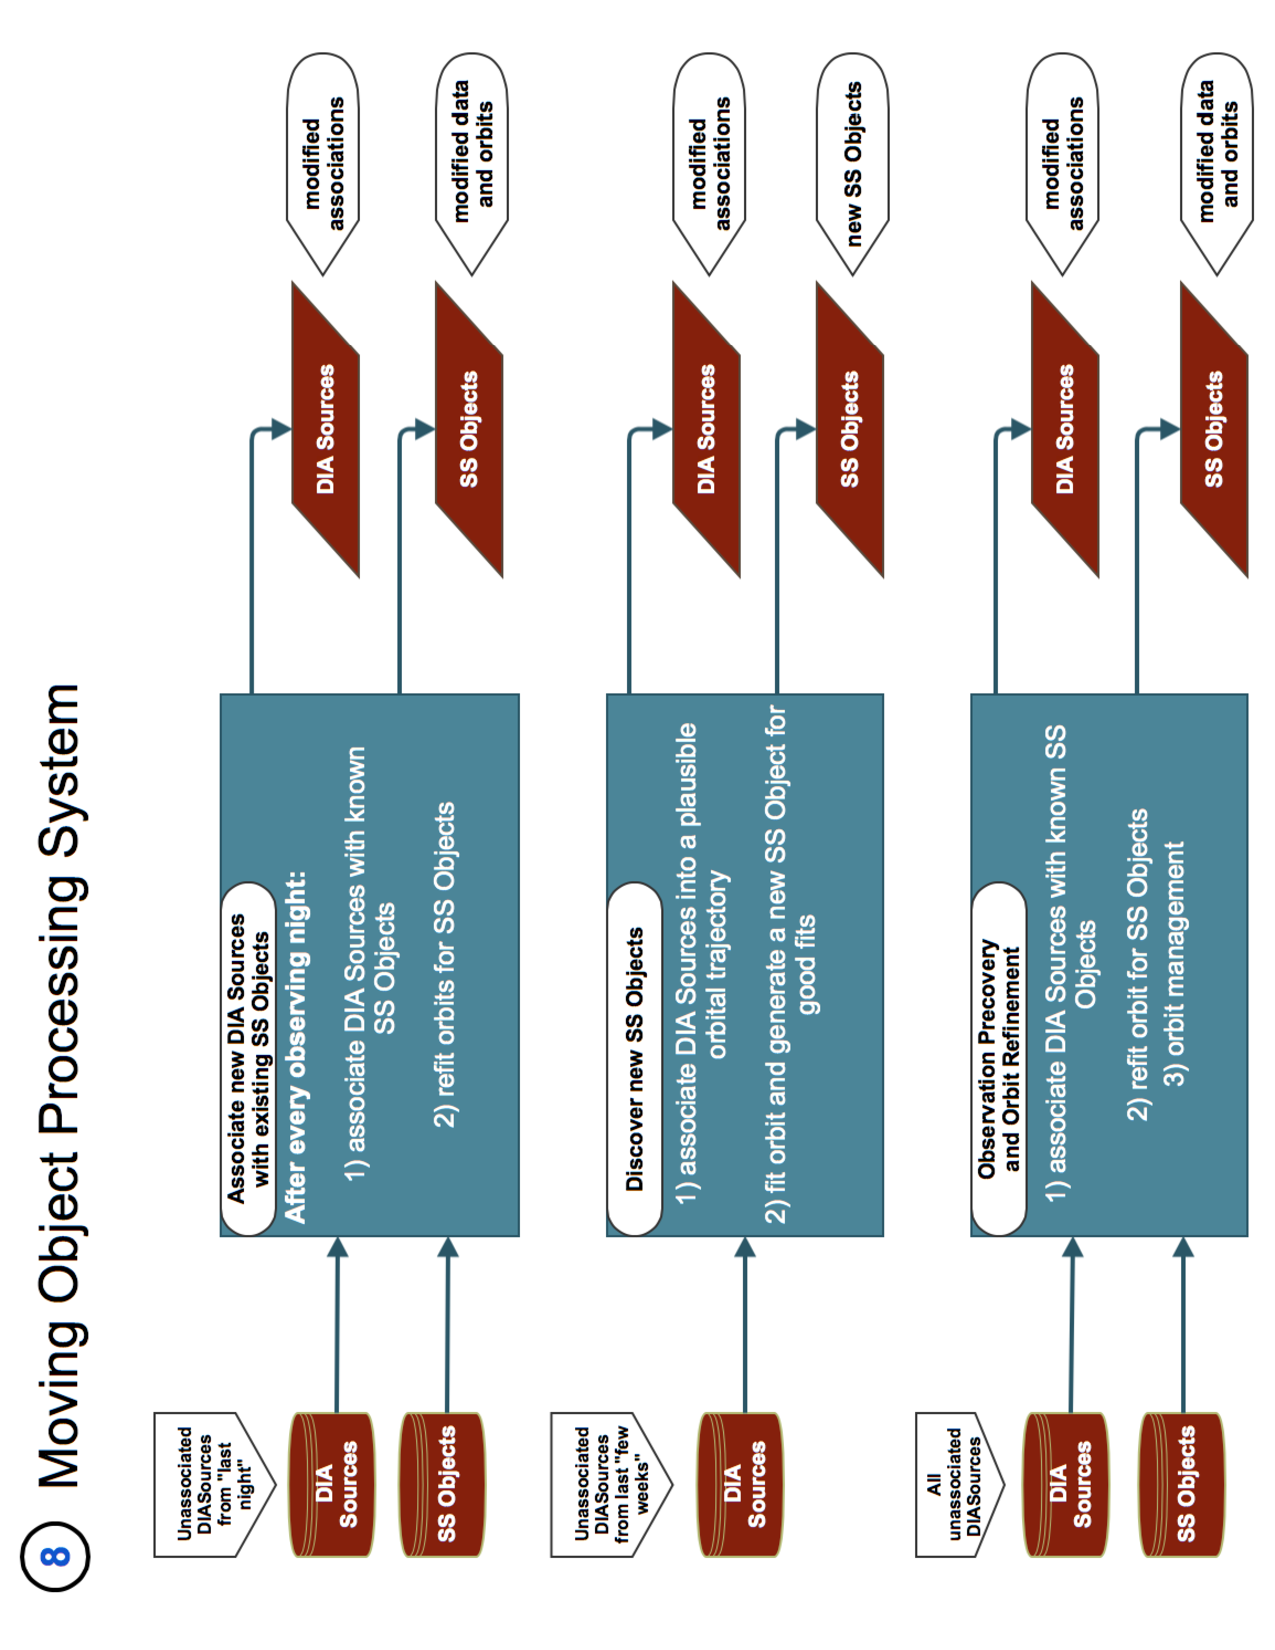
\includegraphics[scale=0.60, angle=270]{MOPS-Level0}
    \vskip -0.1in
    \caption{Illustration of the conceptual algorithm design for the Moving Object Processing System.
   \DIASources are data structures that describe detections of sources in difference images and
   \SSObjects are data structures that describe discovered Solar System objects (see Table~\ref{tab:SSObj}).
\label{fig:Pipe8}}
\end{figure}


\subsection{LSST Level 1 Data Processing}

Level 1 data products are a result of difference image analysis (DIA).
\DIASources are sources detected on difference images with the signal-to-noise ratio $S/N>transSNR$,
with $transSNR$=5.
They represent changes in flux with respect to a deep template. Physically, a \DIASource may be an observation of new astrophysical object that was not present at that position in the template image (for example, an asteroid), or an observation of flux change in an existing source (for example, a variable star). Their flux can be negative (eg., if a source present in the template image reduced its brightness, or moved away). Their shape can be complex (eg., trailed, for a source with proper motion approaching $\sim {\rm deg}/{\rm day}$, or ``dipole-like", if an object's observed position exhibits an offset -- true or apparent -- compared to its position on the template).
Some \DIASources will be caused by background fluctuations; with $transSNR = 5$,
the expected false positive rate is about three per CCD ($\sim 60$ per sq. deg.) for the median seeing,
or of the order 500,000 per typical night.
The expected number of false positives due to background fluctuations is a very strong function
of adopted $transSNR$: a change of $transSNR$ by 0.5
results in a variation of an order of magnitude, and a change of $transSNR$ by unity changes the number of false
positives by about two orders of magnitude.

Clusters of \DIASources detected on visits taken at different times are associated with either a \DIAObject or an \SSObject, to represent the underlying astrophysical phenomenon. The association can be made in two different ways: by assuming the underlying phenomenon is an object within the Solar System moving on an orbit around the Sun\footnote{LSST pipelines will not fit for motion around other Solar System bodies; eg., identifying new satellites of Jupiter is left to the community.}, or by assuming it to be distant enough to only exhibit small parallactic and proper motion\footnote{Where ``small'' is small enough to unambiguously positionally associate together individual apparitions of the object.}. The latter type of association is performed during difference image analysis right after the image has been acquired. The former is done at daytime by \code{MOPS}, unless the \DIASource is an apparition of an already known \SSObject. In that case, it will be flagged as such during difference image analysis. At the end of the difference image analysis of each visit, LSST will issue time domain event alerts for all
newly detected \DIASources\footnote{For observations on the Ecliptic near the opposition Solar System objects will dominate the \DIASource counts and (until they're recognized as such) overwhelm the explosive transient signal. It will therefore be advantageous to quickly identify the majority of Solar System objects early in the survey.}.

\subsubsection{Nightly Difference Image Processing}

The following is a high-level description of steps which will occur during regular {\em nightly}
difference image analysis:
\begin{enumerate}
\item A visit is acquired and reduced to a single {\em visit image} (cosmic ray rejection, instrumental signature removal\footnote{Eg., subtraction of bias and dark frames, flat fielding, bad pixel/column interpolation, etc.}, etc.).
\item The visit image is differenced against the appropriate template and \DIASources are detected and
their properties measured.
\item The flux and shape\footnote{The ``shape'' in this context consists of weighted 2$^{\rm nd}$ moments
of the intensity distribution, as well as fits to a trailed source model and a dipole model.} of the DIASource are measured on the difference image. PSF photometry is performed on the visit image at the position of the \DIASource to obtain a measure of the total flux.
\item The Level 1 database is searched for a \DIAObject or an \SSObject with which to positionally associate the newly discovered \DIASource\footnote{The association algorithm will guarantee that a \DIASource is associated with not more than one existing \DIAObject or \SSObject. The algorithm will take into account the parallax and proper (or Keplerian) motions, as well as the errors in estimated positions of \DIAObject, \SSObject, and \DIASource, to find the maximally likely match. Multiple \DIASources in the same visit will not be matched to the same \DIAObject.}. If no match is found, a new \DIAObject is created and the observed \DIASource is associated to it.
\item If the \DIASource has been associated with an \SSObject (a known Solar System object), it will be flagged as such and an alert will be issued. Further processing will occur in daytime (see \S\ref{sec:ssProcessing} below).
\item Otherwise, the associated \DIAObject measurements will be updated with new data
collected during previous 12 months. All affected columns will be recomputed, including proper motions, centroids, light curves, etc.
\item The \DR\footnote{\DR is a database resulting from annual data release processing.} is searched for \Objects positionally close to the \DIAObject, returning the three nearest stars and three nearest galaxies. The IDs of these nearest-neighbor \Objects are recorded in the \DIAObject record and provided in the issued event alert.
\item An alert is issued that includes the \DIASource ID, the \SSObject ID or \DIAObject ID, and the associated science content (centroid, fluxes, low-order lightcurve moments, periods, etc.), including the full light curves.
\item For all \DIAObjects overlapping the field of view, including those that have an associated
new \DIASource from this visit, forced photometry will be performed on difference image (point source photometry only).
No alerts will be issued for these \DIASources.
\item Within 24 hours of discovery, {\em precovery} PSF forced photometry will be performed on any difference image overlapping the position of new \DIAObjects taken within the past 30 days, and added to the database. Alerts will not be issued with precovery photometry information.
\end{enumerate}

In addition to the processing described above, a smaller sample of sources detected on difference images {\em below} the nominal $transSNR = \transSNR$ threshold will be measured and stored, in order to enable monitoring of difference image analysis quality.

Also, the system will have the ability to measure and alert on a limited\footnote{It will be sized for no less than $\sim 10\%$ of average \DIASource per visit rate.} number of sources detected below the nominal threshold for which additional criteria are satisfied. For example, a $transSNR = 3$ source detection near a gravitational keyhole\footnote{
A gravitational keyhole is a region of space where Earth's gravity would modify the orbit of a passing asteroid
such that the asteroid would collide with the Earth in the future.}
may be highly significant in assessing the danger posed by a potentially hazardous asteroid.
The initial set of criteria will be defined by the start of LSST operations.

\subsubsection{Solar System Object Processing \label{sec:ssProcessing}}

The following will occur during regular Solar System object processing in daytime\footnote{Note that there {\em is no strict bound on when daytime Solar System processing must finish}, just that, averaged over some reasonable timescale (eg., a month), a night's worth of observing is processed within 24 hours. Nights rich in moving objects may take longer to process, while nights with less will finish more quickly. In other words, the system requirement is on {\em throughput}, not latency.}, after a night of observing (see Figure~\ref{fig:Pipe8}):
\begin{enumerate}
\item The orbits and physical properties of all \SSObjects re-observed on the previous night are recomputed. External orbit catalogs (or observations) are also used to improve orbit estimates. Updated data are entered to the \SSObjects table.
\item All \DIASources detected on the previous night, that have {\em not} been matched at a high confidence level to a known \Object,
\DIAObject, \SSObject, or an artifact, are analyzed for potential pairs, forming {\em tracklets}.
\item The collection of tracklets collected over the past 30 days is searched for subsets forming {\em tracks} consistent with being on the same Keplerian orbit around the Sun.
\item For those that are, an orbit is fitted and a new \SSObject table entry created. \DIASource records are updated to point to the new \SSObject record. \DIAObjects ``orphaned'' by this unlinking are deleted.\footnote{Some \DIAObjects may only be left with forced photometry measurements at their location (since all \DIAObjects are force-photometered on previous and subsequent visits);  these will be kept but flagged as such.}.
\item Precovery linking is attempted for all \SSObjects whose orbits were updated in this process. Where successful, \SSObjects (orbits) are recomputed as needed.
\end{enumerate}


\subsubsection{Level 1 Catalogs}
\label{sec:level1db}

The described alert processing design relies on the ``living'' \DB that contains the objects and sources detected on difference images. At the very least\footnote{It will also contain exposure and visit metadata, MOPS-specific tables, etc.}, this database will have tables of \DIASources, \DIAObjects, and \SSObjects, populated in the course of nightly and daily difference image and Solar System object processing\footnote{The latter is also colloquially known as {\em DayMOPS}.}. As these get updated and added to, their updated contents becomes visible (query-able) immediately\footnote{No later than the moment of issuance of any event alert that may refer to it.}.

Table~\ref{tab:SSObj}  presents the {\em conceptual schema} for the \SSObject table (it conveys {\em what} data
will be recorded in each table, rather than the details of {\em how}).
Columns whose type is an array will likely be expanded to one table column per element of the array
once this schema is translated to SQL\footnote{The SQL realization of this schema can be browsed at \url{http://ls.st/8g4}}. In addition, the table presented here is normalized (i.e., it contains no redundant
information with other tables in Level 1 database). For example, since the band of observation can be found
by joining a \DIASource table to the table with exposure metadata, there's no column named {\tt band} in the \DIASource table. In the as-built database, the views presented to the users will be appropriately denormalized
for ease of use.

\subsubsection{\SSObject Table}

\begin{center}
\label{tab:SSObj}
\begin{longtable}{p{3cm}p{2cm}p{2cm}p{5cm}}
%\caption[\SSObject Table]{\SSObject Table} \\

\hline \multicolumn{1}{c}{\bf Name} & \multicolumn{1}{c}{\bf Type} & \multicolumn{1}{c}{\bf Unit} & \multicolumn{1}{c}{\bf Description} \\ \hline
\endhead

\hline \multicolumn{4}{r}{{\em Continued on next page}} \\
\endfoot

\hline\hline
\endlastfoot

ssObjectId & uint64 & ~ & Unique identifier. \\

oe & double[7] & various & Osculating orbital elements at epoch ($q$, $e$, $i$, $\Omega$, $\omega$, $M_0$, epoch). \\

oeCov & double[21] & various & Covariance matrix for \texttt{oe}. \\

arc & float & days & Arc of observation. \\

orbFitLnL & float & ~ & Natural log of the likelihood of the orbital elements fit. \\

orbFitChi2 & float & ~ & $\chi^2$ statistic of the orbital elements fit. \\

orbFitNdata & int & ~ & The number of data points (observations) used to fit the orbital elements. \\

MOID & float[2] & AU & Minimum orbit intersection distances\footnote{\url{http://www2.lowell.edu/users/elgb/moid.html}} \\

moidLon & double[2] & degrees & MOID longitudes. \\

H & float[6] & mag & Mean absolute magnitude, per band (Muinonen et al. 2010 magnitude-phase system). \\

${\rm G_1}$ & float[6] & mag & $G_1$ slope parameter, per band (Muinonen et al. 2010 magnitude-phase system). \\

${\rm G_2}$ & float[6] & mag & $G_2$ slope parameter, per band (Muinonen et al. 2010 magnitude-phase system). \\

hErr & float[6] & mag & Uncertainty of H estimate.\\

g1Err & float[6] & mag & Uncertainty of $G_1$ estimate. \\

g2Err & float[6] & mag & Uncertainty of $G_2$ estimate. \\

flags & bit[64] & bit & Various useful flags. \\ \hline

\end{longtable}
\end{center}

The $G_1$ and $G_2$ parameters for the large majority of asteroids will not be well constrained until later in the survey. LSST may decide not to fit for it at all over the first few DRs and add it later in Operations, or provide two-parameter $G_{12}$ fits. Alternatively, they may be fitted using strong priors on slopes poorly constrained by the data. The design of the data management system is insensitive to this decision, making it possible to postpone it to Commissioning to ensure it follows the standard community practice at that time.
The LSST database will provide functions to compute the phase (Sun-Asteroid-Earth) angle $\alpha$ for every observation, as well as the reduced, $H(\alpha)$, and absolute, $H$, asteroid magnitudes in LSST bands.

\section{The Impact of False Positives on MOPS Performance \label{sec:appMOPS}}


We seek to develop an analytic understanding for the behavior of the MOPS results.
In particular, we want to be able to predict the numbers of tracklets and
candidate tracks for a given input number of true and false detections. In addition, we seek
to understand how these numbers scale with the search window width,
velocity cutoff when forming tracklets, the temporal separation of two
detections in a tracklet, and the density of false positives. For example, available
MOPS experiments indicate that the number of tracklets increases with
the square of the false positives density, but other scalings are unclear,
especially the behavior of false candidate tracks.

We first derive the simpler false tracklet rates, and then use these results to
discuss false candidate track rates.


\subsection{Expected False Tracklet Rates \label{sec:tracklets} }

Given a detection in the first difference image,  another difference image, obtained at a different epoch,
is searched for a matching detection to form a tracklet. For orientation,
the sky density of asteroids down to LSST $5\sigma$ faint flux limit ($r \sim 24.5$) is of the order
$\rho_{ast} \sim 100$ deg$^{-2}$. The predicted highest asteroid sky density for $r<24.5$,
on the Ecliptic, is up to about five times larger (with an uncertainty of about a factor of 2,
depending on model assumptions), and the density decreases rapidly with the ecliptic latitude.
A typical LSST observing night includes about 1000 visits, with two visits per night over
the active sky area. The nominal LSST field-of-view area is $A_{FOV}=9.6$ deg$^2$, with a
fill factor of 0.9, giving an effective field-of-view area of $A_{FOV}^{eff}=8.64$ deg$^2$. Hence,
the number of detected asteroids per night is of the order 500,000 (with implied two detections
per asteroid), although it can be significantly lower when the Ecliptic is not well covered (and
it could be a few times higher if the majority of visits were obtained along the Ecliptic).

The number of false detections due to (Gaussian) background fluctuations is
about $\rho_{bkgd} = 60$ deg$^{-2}$, assuming typical LSST seeing (0.8 arcsec)
and SNR$>$5. For a given seeing and SNR threshold, the rate of false positives can never be
lower than this estimate. This false positive rate decreases with the square of the seeing, and
strongly depends on SNR: the rate increases/decreases by as much as a factor of about ten
when SNR threshold is changed to 4.5 and 5.5, respectively (see \S\ref{sec:imDiff}).

Analysis of DECam images reduced using prototype LSST software, described in \S\ref{sec:imDiff},
shows a higher rate of detections in difference images, and a fraction of those detections
cannot be readily associated with true moving objects. This analysis implies a conservative
upper limit for the false positive rate of about $\rho_{FP} =  400$ deg$^{-2}$. This value
is conservative because analyzed DECam fields are close to the Ecliptic, with a significant but
not well known contribution from real asteroids (due to very faint flux levels, $r \sim 24$),
and it also includes true astrophysical transients that are not associated with static objects
(stars and galaxies). It is quite possible that the false positive rate might be several
times lower, though we will proceed with the most conservative estimate above.

The sky density of detections in difference images, $\rho_{det}$, is given by
the sum of contributions from true asteroids and false positives, $\rho_{det} = \rho_{ast} + \rho_{FP}
= 500$ deg$^{-2}$. When searching for a matching detection in another difference image, there are
two distinct types of behavior. Correct matches of detections of the same asteroids into tracklets follow the behavior
expected for correlated samples: as long as the object's angular displacement between the two epochs
is sufficiently larger than the seeing disk, while at the same time smaller than the search radius, the
number of matches (that is, the number of true tracklets produced per LSST pointing, assuming
two visits of the same area per night) is simply
\begin{equation}
                  N_{tracklet}^{true} = \rho_{ast}  \, A_{FOV}^{eff},
\end{equation}
With  $\rho_{ast} = 100$ deg$^{-2}$, $N_{tracklet}^{true} \sim 1,000$ per a pair of visits, and with
500 visit pairs per typical observing night, $N_{tracklet}^{true} \sim 500,000$ per night (same as
the number of detected asteroids in the active sky area, of course). Again,
this number can be much lower for fields far away from the Ecliptic, and a few times larger
for exceptionally good coverage of the Ecliptic. We emphasize that this number of true tracklets
does not directly depend on the search radius, nor the time elapsed between the two visits, as long
as they have their plausible values (about an arcminute, and a few tens of minutes, as discussed
further below).


\begin{figure}[t!]
\centering
\vskip -2.0in
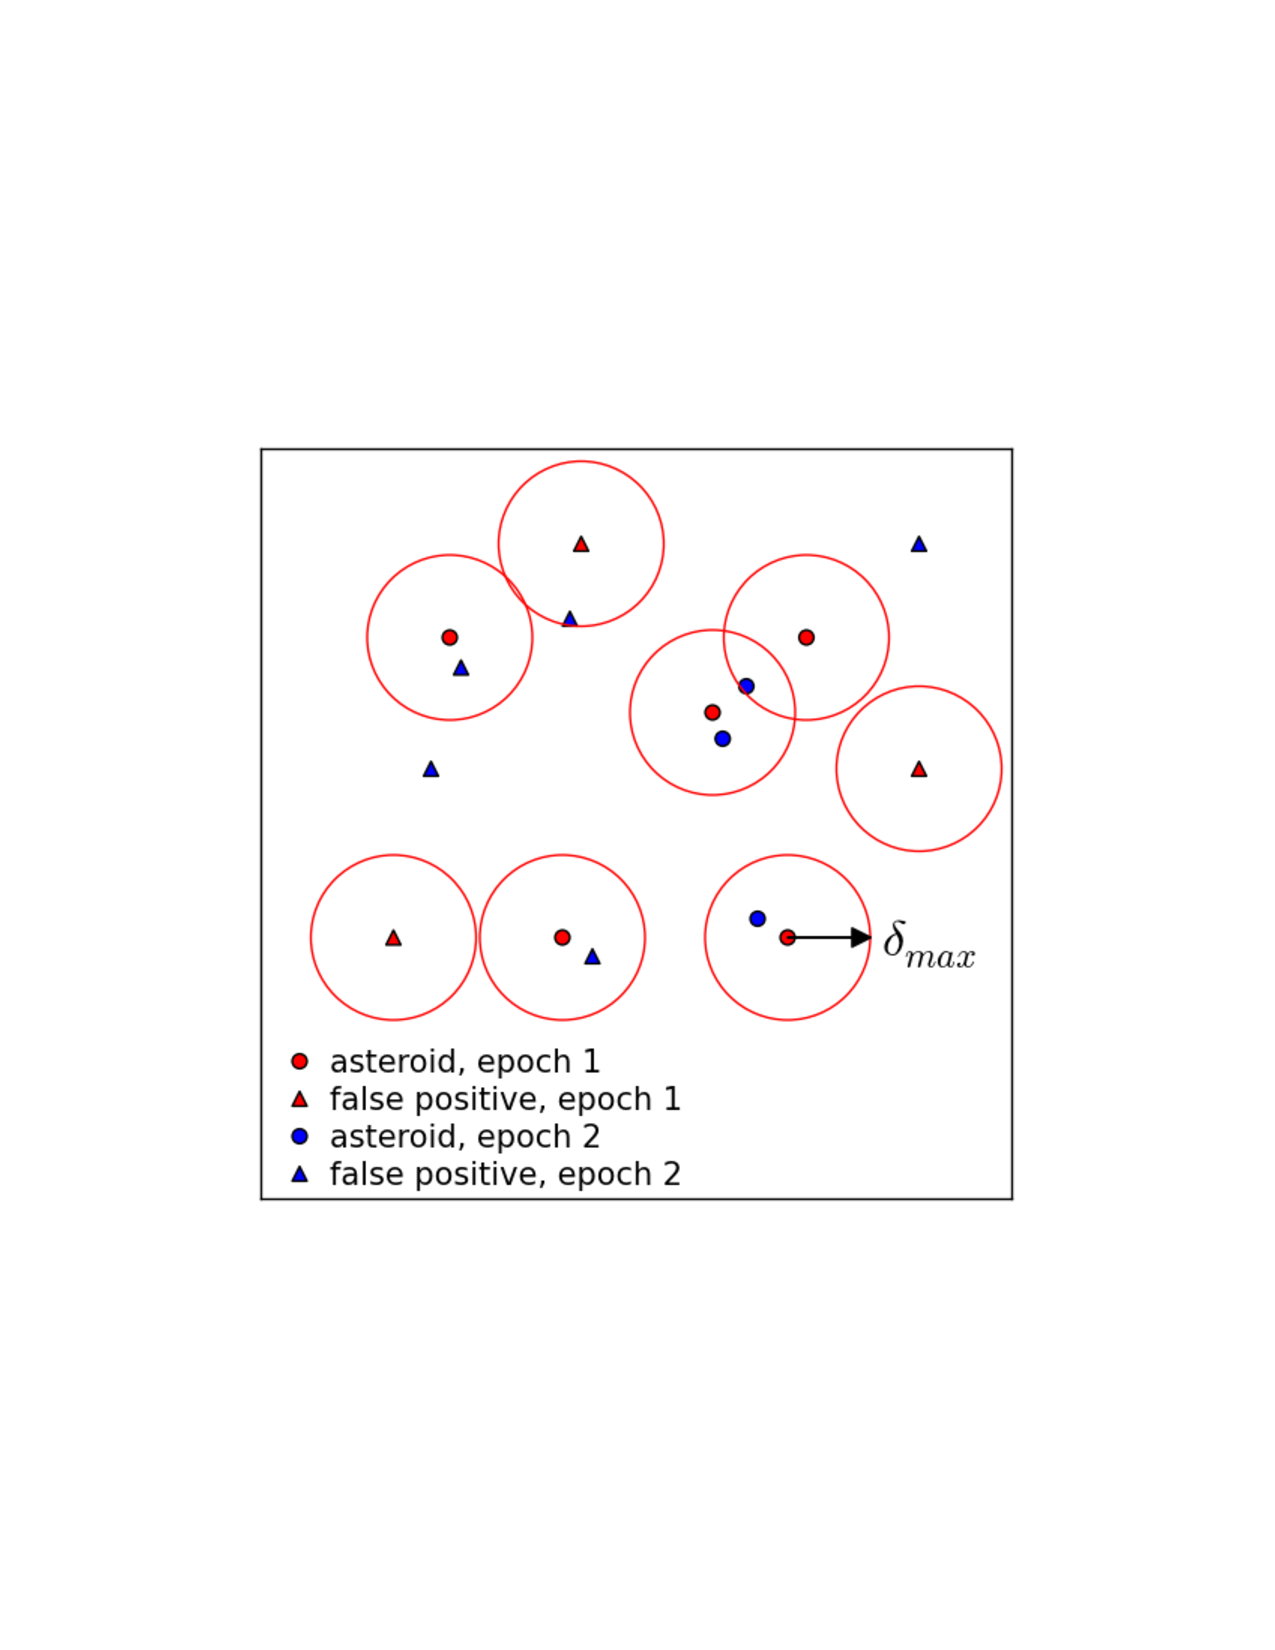
\includegraphics[width=0.95\textwidth]{figures/TrackSlide2}
\vskip -2.2in
\caption{An illustration of positional matching of detections to form tracklets.
Detections come in two flavors: asteroids (A, circles) and false positives (FP, triangles).
The figure shows the search for a matching detection in epoch 2 for each detection
in epoch 1, with a maximum search radius $\delta_{max}$. Note that there are six
possibilities: matches A-A, A-FP, FP-A, FP-FP, and orphaned A and FP.
\label{fig:TrackSlide2}}
\end{figure}

There are three other types of tracklets that follow behavior for uncorrelated (random)
samples: associations of different asteroids, associations of asteroids and false detections,
and tracklets made of two false detections. Assuming the same $\rho_{det}$ in both
difference images, for each of $N_{det} = \rho_{det} \, A_{FOV}^{eff}$ detections in one image,
we search for a matching detection in another image (see Figure~\ref{fig:TrackSlide2}).
The search radius is given by
\begin{equation}
                     \delta_{max} = v_{max} \, \Delta t .
\end{equation}
Here $v_{max}$ is the  cutoff velocity and $\Delta t$
is the time elapsed between the two images. For LSST baseline cadence, $\Delta t$ is in
the range 20-60 minutes. The search area, $A_S = \pi \delta_{max}^2$, is then
\begin{equation}
\label{eq:AS}
      A_S = 0.0055 \left( v_{max}  \over {\rm deg \, day}^{-1} \right)^2 \, \left(\Delta t \over {\rm hour} \right)^2 {\rm deg}^2.
\end{equation}
To guide setting the cutoff velocity, simulations imply that 95\% of NEO detections have $v<1$ deg day$^{-1}$; with this threshold,
the completeness for main-belt asteroids is essentially 100\%. Objects moving faster than 1 deg day$^{-1}$ will
be easily resolved in LSST images and can be treated separately using specialized algorithms.
Adopting $v_{max} = 1$ deg day$^{-1}$,  and $\Delta t = 30$
minutes (which together  imply a search radius of $\delta_{max} = 1.3$ arcmin), gives a search area of
$A_S = 0.0014$ deg$^2$.


The expectation value for the number of matching detections within the search area $A_S$ (that is, the expected
number of tracklets per matching trial) is
\begin{equation}
                      p_{tracklet}^{false} =   \rho_{det}  \, A_S,
\end{equation}
and the total expected number of {\it false} tracklets for $N_{det}$ trials is thus
\begin{equation}
\label{eq:NttFalse}
           N_{tracklet}^{false} = N_{det} \, p_{tracklet}^{false} =  N_{visit} \, \rho_{det}^2 \, A_S \, A_{FOV}^{eff} = N_{visit} \, \rho^2_{FP}  \, A_S \, A_{FOV}^{eff} \,  \left(1 + 2 \eta + \eta^2\right),
\end{equation}
where $\eta = \rho_{ast}  / \rho_{FP} \sim 0.25$ (recall that $\rho_{det} = \rho_{ast} + \rho_{FP}$).
With $\rho_{ast} = 100$ deg$^{-2}$ and  $\rho_{FP} = 400$ deg$^{-2}$,
$N_{tracklet}^{false} \sim 3,000$ per pair of visits, and $N_{tracklet}^{false} \sim 1.5$ million per observing night with
$N_{visit}=500$ visit pairs. We note that the density of false tracklets ($\rho_{tracklet}^{false}=350$ deg$^{-2}$) is similar to
$\rho_{FP}$; this similarity is a consequence of choosing $\delta_{max}$ such that $\rho_{FP} A_S \sim 1$.

The first term in eq.~\ref{eq:NttFalse} is the largest and corresponds to tracklets made of two false
detections ($\sim1.0$ million), the second term corresponds to associations of asteroids and false detections,
and the third and the smallest term ($<0.1$ million) is due to incorrect associations of different asteroids.
For the chosen parameter values, the total number of tracklets is about 2 million per observing night, Given that
these choices are rather conservative, this estimate is essentially an upper limit; approximately,
{\it we expect of the order a million tracklets per observing night}.

To the first order ($\eta \approx 0$), the total number of tracklets per night is
\begin{equation}
    N_{tracklet} =  N_{tracklet}^{true} + N_{tracklet}^{false} =
       N_{visit} \, A_{FOV}^{eff} \, \left(\rho_{ast}  + \rho^2_{FP}  \, A_S \right).
\end{equation}
In addition to $N_{tracklet}^{false}$ scaling with the square of $\rho_{FP}$, as demonstrated using MOPS,
$N_{tracklet}^{false}$ scales with the square of
both $v_{max}$ and  $\Delta t$ (via the dependence on $A_S$). Therefore, if $\Delta t$ would be made
as small as 10 minutes by modifying observing strategy, the resulting $N_{tracklet}^{false}$ would be about an
order of magnitude smaller (and $N_{tracklet}$ about three times smaller).  Hence, the shortening of $\Delta t$ is
a good mitigation strategy against high false positive detection rates in difference images\footnote{An
extreme example of this mitigation strategy would be to obtain two consecutive 30-second visits -- their
mid-exposure times would be separated by 34 seconds (additional 2 seconds due to shutter motion and another
2 seconds due to readout), which is sufficient to detect motion faster than about 0.1 deg day$^{-1}$.}.


\subsubsection{False tracklet velocity distribution \label{sec:falsev}}

False tracklets have randomly distributed velocities (motion vectors) with a cutoff given by $v_{max}$
(recall that $v_{max} = 1$ deg day$^{-1}$ was adopted above). The implied tracklet velocity is given by
\begin{equation}
                       v =  \delta / \Delta t,
\end{equation}
where $\delta$ is the angular separation of two detections. Since the number of tracklets
with separation $\delta$ increases linearly with $\delta$ (because the area of a circular
annulus is $2\pi r dr$), the false tracklet velocity distribution will increase linearly with
$v$ for $v<v_{max}$, and the vector orientation will be random. We show below that candidate
tracks can be efficiently pruned using this result.



\subsection{Expected False Track Rates \label{sec:tracks} }

In this section, we present an approximate estimate of the expected number of false candidate tracks.
Our goal is to derive the scaling of this number with relevant input parameters, such as the true and false
tracklet rates per night ($N_{tracklet}^{true}=5\times10^5$ and $N_{tracklet}^{false}=1.5\times10^6$, respectively).
For a fiducial case, we assume that the search window is $N_w= 30$ days wide;  therefore, with $N_{tracklet} = 2\times10^6$
per night, there are $6\times10^7$ tracklets in the fiducial dataset. With about 4,300 deg$^2$ (500 pairs of visits)
of sky observed each night, the average density of (all) tracklets is $\rho_{tracklet} = 450$ deg$^{-2}$. Assuming
that on average the same field is revisited every $T_{revisit}=3$ days, the active area includes about 13,000 deg$^2$
of sky.

As discussed below in more detail, there are of the order 1000 different ways to chose a triplet of nights
from the search window. Given 10$^6$ tracklets per night, there are of the order
10$^{21}$ different combinations of tracklet triplets that could form a candidate track.
While this number of candidate tracks is obviously prohibitively large to test for consistency
with heliocentric Keplerian motion, it can be sufficiently reduced (to about the same number
as the number of true tracks along the Ecliptic) using pre-filtering steps based on tracklet motion
vectors, as follows.

In the first step, the motion vector of a tracklet from the first night is linearly extrapolated
to the second night and tracklets from the second night are searched for within a radius set
by the orbital curvature (which dominates over astrometric errors). With appropriate use of
kd-tree and similar algorithms for fast searches, only a small fraction (of the order a percent)
of tracklets from the second night need to be examined in detail. The cutoff radius varies
from $\sim$1 arcmin for the case of two consecutive nights to $\sim$1 deg. for 15-day separation
(as discussed in detail further below). In addition, the velocity of second tracklet is required
to be consistent with the velocity implied by the positions of the two tracklets. After
this step, there are about 10$^{10}$ tracklet pairs for further processing (for $N_w=30$
days).

In the second step, parameters of a parabola (for each coordinate) are constrained using the
positions and velocities of the two tracklets, and this parabolic motion is extended to a third
night to search for matching third tracklet. This step results in up to 10$^{11}$ candidate
tracks.

Using positions of the three tracklets, parabolic motion (for each coordinate) is fit
in the third step. Velocities implied by this motion fit are compared to velocities for
the first and third tracklet. This filtering step reduces the number of candidate tracks
by a factor of about 10$^{-5}$ and brings the number of false candidate tracks to
the same range as the number of true tracks close to the Ecliptic. These three matching
and pre-filtering steps bring the number of candidate tracks to a level that
can be easily handled by the IOD filtering step.

We now proceed with a more detailed description of  three pre-filtering steps
for candidate tracks.

\subsubsection{The Number of 3-night Combinations in the Search Window}

We can form a candidate triplet of tracklets by first choosing the middle (second) tracklet.
For simplicity, we will measure time of observation in integer days. Given $N_w$ nights
in the search window, the middle tracklet comes from night indexed $k$, with
$2 \le k \le (N_w-1)$. The night that contributes the first tracklet is indexed by $j$,
with $1 \le j \le (k-1)$, and the night that contributes the third tracklet is indexed by $l$,
with $(k+1) \le l \le N_w$. The number of 3-night combinations can be expressed in a closed
form
\begin{equation}
\label{eq:N3}
  N_{3nights} = \sum_{k=2}^{N_w-1} \, (k-1)\, (N_w-k) =\frac{1}{6}N_w^3 - \frac{1}{2}N_w^2 + \frac{1}{3}N_w,
\end{equation}
giving $N_{3nights} = 455$ for $N_w=15$ and $N_{3nights} = 4,060$ for $N_w=30$.  Note
that for large $N_w$, $N_{3night}$ is proportional to $N_w^3$ -- the number of 3-nights
combinations increases by about an order of magnitude when $N_w$ is doubled from
15 days to 30 days.

It is important to point out that in steady-state processing a single night is added to the
window from the previous night, and the first night is dropped. Therefore, only the {\it new}
3-night combinations, where the third night is the last night in the search window, need
be considered in steady-state processing (and the ramp up is easy because of gradually
increasing search window size). It is straightforward to show that the number of such
3-night combinations is
\begin{equation}
\label{eq:N3n}
  N_{3nights}^{new} = \sum_{k=2}^{N_w-1} \, (k-1) =\frac{1}{2}N_w^2 - \frac{3}{2}N_w + 1,
\end{equation}
yielding $N_{3nights}^{new} = 91$ for $N_w=15$ and $N_{3nights}^{new} = 406$ for $N_w=30$.
Note that $N_{3nights}^{new} \sim N_{3nights} / 10)$ for $N_w=30$, which represents
a significant reduction.


\subsubsection{The Tracklet Motion Vector Accuracy \label{sec:astromerrors}}

In addition to its mean position at the mean epoch, each tracklet constrains the motion vector.
Typical astrometric errors for LSST detections will range from about 50 mas at SNR=100 to
150 mas at SNR=5. For simplicity, we will assume hereafter that the astrometric errors are
$\sigma_a=150$ mas for all detections, or $\sim 100$ mas per coordinate. With a temporal
separation of two detections in a tracklet of $\Delta t$, the motion vector is measured with an
accuracy per coordinate of
\begin{equation}
\label{eq:sigv}
          \sigma_v = 3.6 \, \left({\rm hour} \over \Delta t\right) \,\,\, {\rm arcsec} \, {\rm day}^{-1}.
\end{equation}
With a typical $\Delta t = 30$ min, and assuming a linear motion in each ecliptic coordinate (longitude
$\lambda$ and latitude $\beta$), each coordinate can be predicted at time $t$ with an accuracy of
\begin{equation}
            \sigma_x = 7.2 \, \Delta k \,\,\, {\rm arcsec},
\end{equation}
where $\Delta k$, in days, is the elapsed time between the mean tracklet epoch and time $t$
(for example, the number of nights between the first and the second tracklet in a candidate track).
For illustration, when $\Delta k = 7$ days, $\sigma_x = 50$ arcsec, which is roughly the same
as the typical detection separation in a tracklet, and comparable to typical distance between
two tracklets.  However, it turns out that positional discrepancies due to linear extrapolation of
orbital motion for NEOs are an order of magnitude larger than the astrometric measurement errors
even in case of two consecutive nights ($\sim$1 arcmin vs. 7 arcsec, respectively). We proceed with
a quantitative analysis of required matching radius using simulated orbits for main-belt asteroids
and NEOs.



\subsubsection{Initial Linking of Tracklets into Candidate Tracks}

Given a combination of 3 different nights from the search window, for each tracklet
from the first night we can linearly extrapolate its motion vector and require that the
measured  position of a tracklet from the second night is consistent with the predicted
position (the night ordering can be reversed from 1-2-3 to 3-2-1). Given a tracklet from
the first night, it is not necessary to search through all tracklets from the second night.
Search methods such as kd-trees can be used to rapidly reject tracklets that have no
chance of being matched. As an example of a ``poor man's'' rapid search, consider the
fact that tracklets from each night are already ``self-organized'' into about 500 visits,
which correspond to a field of view with a diameter of 3.5 deg. It is easy to show that with
an upper limit on possible motion of 5 deg, only 19 visits from the second night need to be
searched for matching  tracklets. This significant reduction of a factor of $\sim$25 in
the number of candidate matching tracklets can be further boosted by applying more
sophisticated tree algorithms.

Using for illustration ecliptic longitude $\lambda$, the predicted search position for the
second tracklet is
\begin{equation}
\label{eq:lambdaPred}
               \lambda_2^\ast = \lambda_1 + v_1^\lambda \, \Delta T_{21},
\end{equation}
where $\Delta T_{21}$ is the elapsed time between the epochs of the first and second tracklet,
and $v_1^\lambda$ is the longitudinal component of $v_1$, the motion vector for the first
tracklet, {\it divided by} cos($\beta$). The expectation value for the number of matches in
an ellipse (see the left panel in Figure~\ref{fig:TrackSlide1})
centered on predicted position ($\lambda_2^\ast, \beta_2^\ast$), and within limits $r_\lambda^{max}$
and  $r_\beta^{max}$ along the Ecliptic longitude and latitude, is given by
\begin{equation}
\label{eq:Nmdk}
     N_{match}(\Delta k) = \pi \, r_\lambda^{max} \, r_\beta^{max}  \, \rho_{tracklet} \left({1 \, {\rm day} \over T_{revisit}}\right)
\end{equation}
where division by $T_{revisit}$ reflects the fact that each field is revisited on average only
every $T_{revisit}$ days (statistically speaking; the number of matches is zero for all but one
night out of $T_{revisit}$ nights).

The extrapolation given by eq.~\ref{eq:lambdaPred} implies that orbits can be approximated by
linear motion (in each coordinate) over time $\Delta T$. This is an incorrect assumption
due to orbital curvature and we analyze this effect using orbital simulations of MBA and NEO
samples described in \S\ref{sec:MAFdetails}.

Analysis of simulated samples shows that an adequate acceleration limit\footnote{See also
Figure 16 in \citet{LDM-156}} is $a^{max}=0.02$ deg day$^{-2}$: essentially
all main-belt asteroids and more than 95\% of NEOs satisfy this criterion. If acceleration
were constant during an interval of $\Delta k$ days, the maximum positional discrepancy
would be proportional to $\Delta k^2$. Numerical analysis of simulated orbital motions
suggests that an approximately constant selection completeness (as a function of $\Delta k$)
is attained for
\begin{equation}
\label{eq:matching1}
                r_\beta^{max} = A \, \Delta k^{1.5}.
\end{equation}
with $A=1.0$ arcmin, and $r_\lambda^{max} = 5 \, r_\beta^{max}$. The achieved completeness for
a fiducial $\Delta k$=7 days is 0.99 for MBAs and 0.95 for NEOs, with very little dependence
on $\Delta k$ for 1 day $\le \Delta k \le$ 21 days (per single search window -- note that most
objects will have multiple discovery chances).  With this linear motion model, the number
of matched tracklets per single trial tracklet is
\begin{equation}
\label{eq:Nmdk2}
   N^{L}_{match}(\Delta k) = 1.96 \, \left({1 \, {\rm day} \over T_{revisit}}\right) \,
                    \left( \rho_{tracklet}  \over 450 \, {\rm deg}^{-2} \right) \, (\Delta k)^3.
\end{equation}
For example,  the expected number of matches for $\Delta k$=7 days is $\sim$224
(a 19 arcmin by 93 arcmin matching ellipse), and rises to $\sim$6,000 for
$\Delta k$=21 days.

Given the two matched tracklets, we approximate the motion as a parabola
\begin{equation}
\label{eq:parabola}
          \lambda(t) = \frac{1}{2}a^\lambda \, t^2 + v^\lambda \, t + \lambda_1,
\end{equation}
where $t = mjd - mjd_1$ (and analogously for latitude $\beta$).  Using the tracklet
positions and the motion vector of the first tracklet, acceleration can be directly
estimated as
\begin{equation}
 \label{eq:accPred}
             a^\lambda = 2 \, {\lambda_2- \lambda_1 - v_1^\lambda \Delta T_{21} \over \Delta T^2_{21}},
\end{equation}
and the predicted velocity for the second tracklet can be estimated from
\begin{equation}
\label{eq:v2cut}
        (v^\lambda_2)^\ast =  a^\lambda \,\Delta T_{21}  + v_1^\lambda =
      {2(\lambda_2- \lambda_1) \over \Delta T_{21}}  - v_1^\lambda.
\end{equation}

We find that a comparison of $v_2^\lambda$ and $(v^\lambda_2)^\ast$ can further decrease
the number of false tracks (recall \S\ref{sec:falsev}); with tolerances of $\Delta v^\lambda < 0.3$ deg/day and
$\Delta v^\beta < 0.07$ deg/day (applied simultaneously for both coordinates as an
elliptical condition), the reduction is about a factor of 50 (for $v_{max}$ = 1 deg day$^{-1}$),
with only a minimal impact on the sample completeness. Therefore, depending on $\Delta k$, the number of tracklet
pairs per trial tracklet  to continue processing ranges from $\sim$4 for $\Delta k$=7 days to
$\sim$120 for $\Delta k$=21 days. When added over all possible pairs of nights (with
$T_{revisit}=3$ days), the total number of candidate tracklet pairs normalized by
the number of tracklets per night ranges from 350 for $N_w=15$ days to 13,400 for $N_w=30$ days.
Therefore, the following, more involved, selection steps need to be executed for
no more than about $10^{10}$ tracklet pairs (for $N_w=30$ days; and only for $3\times10^{8}$
pair when $N_w=15$ days). These numbers are significantly lower than the naive estimate of
10$^{15}$ ($10^3\times10^6\times10^6$).

We note that in steady-state processing, the new candidate tracklet pairs need to
be evaluated only for pairs of nights where the second night is the penultimate
night in the search window (all other combinations will have been already computed
on previous days). Because the caching of results from previous night is not
yet implemented in MOPS, we don't account for this reduction (of about a factor of
3 to 6) in the analysis presented here.

Given the acceleration estimate from eq.~\ref{eq:accPred}, the position of the third
tracklet can be predicted from
\begin{equation}
\label{eq:lambdaPred3}
  \lambda_3^\ast = \frac{1}{2} a^\lambda \, \Delta T_{32}^2 + v_2^\lambda \, \Delta T_{32} + \lambda_2.
\end{equation}
Similarly to eq~\ref{eq:matching1}, an approximately constant selection completeness
can be achieved using
\begin{equation}
\label{eq:matching2}
                r_\beta^{max} = B \, \Delta k^{1.5}.
\end{equation}
with $B=0.2$ arcmin, and $r_\lambda^{max} = 5 \, r_\beta^{max}$. Note that the search
area is now 25 times smaller than in the first case, thanks to parabolic rather
than linear extrapolation. Therefore, the number of matched tracklets per single
trial tracklet pair is
\begin{equation}
\label{eq:Nmdk3}
     N^P_{match}(\Delta k) = 0.078 \, \left({1 \, {\rm day} \over T_{revisit}}\right) \,
                    \left( \rho_{tracklet}  \over 450 \, {\rm deg}^{-2} \right) \, (\Delta k)^3,
\end{equation}
and the expected number of matches ranges from 9 for $\Delta k$=7 days to
$\sim$240 for $\Delta k$=21 days.

%####
The total number of candidate tracks per single trial tracklet, for all possible 3-night
combinations (where the third night is the last night in the search window) is
\begin{equation}
\label{eq:Ntt}
   N_{tracklet}^{tracks} = 3.2\times10^{-3} \, \left( \rho_{tracklet}  \over 450 \, {\rm deg}^{-2} \right)^2 \, \left({1 \,{\rm day}\over T_{revisit}}\right)^2 \, \sum_{k=2}^{N_w-1} \sum_{j=1}^{k-1} \, (k-j)^3 \, (N_w-k)^3.
\end{equation}
The normalization constant is equal to $1.96\times0.078\times(\Delta v^\lambda
\Delta v^\beta/v_{max}^2)$, where the term in parenthesis is $\sim0.02$. This
normalization gives the number of candidate tracks per search window normalized
by the number of tracklets per night (which is assumed constant for all nights).
The two terms in the sum reflect the multiplication of the number of matches found
in the first selection step (linear extrapolation from the first to the second night,
eq.~\ref{eq:Nmdk2}) and the number of matches found in the third selection step
(parabolic extrapolation from the second to the third night, eq.~\ref{eq:Nmdk3}).

The sums in eq.~\ref{eq:Ntt} can be evaluated analytically, but the result is cumbersome.
Using numerical evaluation (with $T_{revisit}=3$ days), we find that the number of candidate
tracks per tracklet ranges from $\sim600$ for $N_w=15$ days to $\sim174,000$ for
$N_w=30$ days ($N_{tracklet}^{tracks}$ scales with $N_w^8$ when the third night must be
the last night from the search window).
Therefore, the matching of the candidate third tracklet brings the number of candidate
tracks per search window to the range 10$^{9}$ - 10$^{11}$. The ratio of false candidate tracks
to true tracks is in the range 10$^{3}$ - 10$^{5}$, depending on $N_w$. Despite the reduction by
a factor of  about $10^{10}$ to $10^{12}$ from the combinatorial number of tracklet triplets,
another significant reduction is required before the IOD step can be attempted.


\begin{figure}[th!]
\centering
\vskip -2.6in
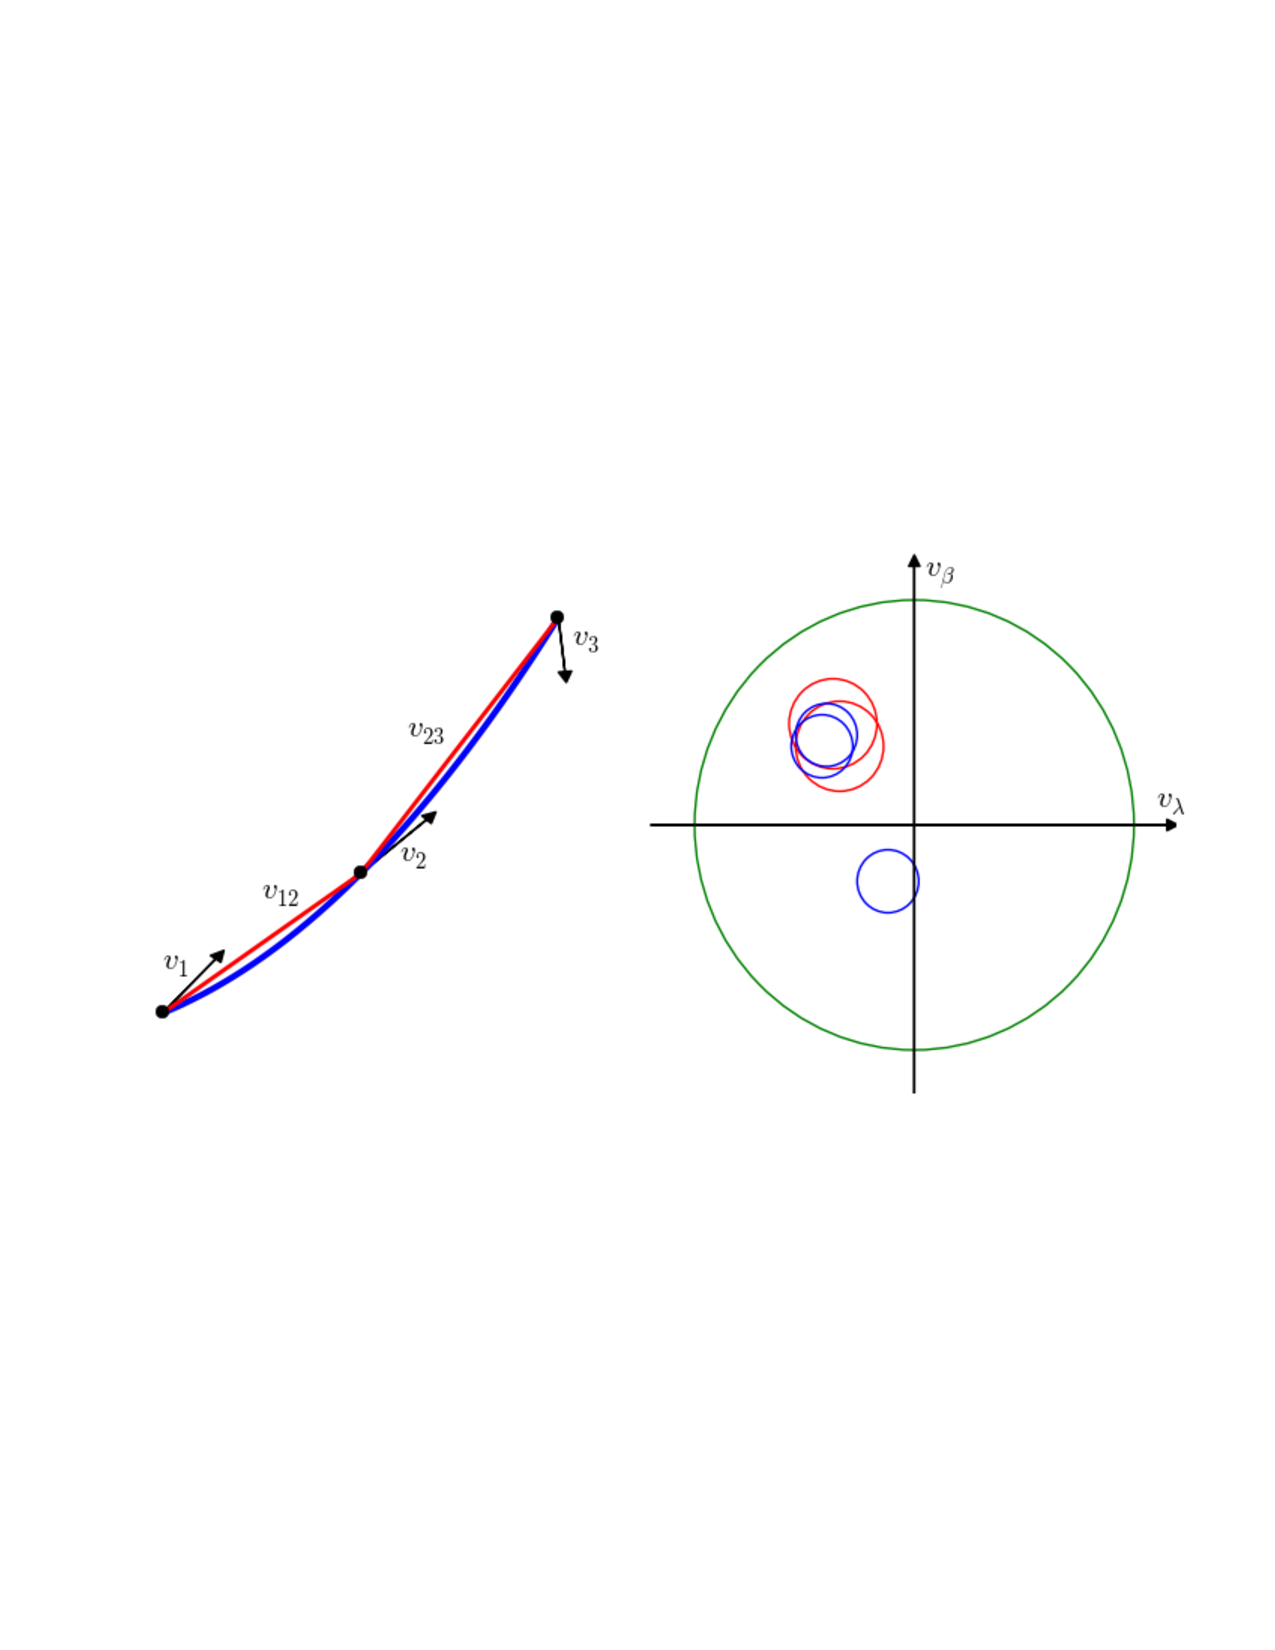
\includegraphics[width=0.95\textwidth]{figures/TrackSlide1}
\vskip -2.7in
\caption{The left panel shows a hypothetical asteroid trajectory as the curved blue line (with
the curvature greatly exaggerated). Three tracklets are shown by the black dots; the
two individual detections per tracklet are not shown, but are implied by the three measured
motion vectors ($v_1$, $v_2$ and $v_3$). The third tracklet illustrates a false tracklet.
The motion vector of the first tracklet is linearly extrapolated to the time of the second
tracklet and matched within the red ellipse. The first two tracklets are then used to
constrain parabolic extrapolation, shown by the green dotted line, which is then matched
within the green ellipse. Given three candidate tracklets, a parabola is fit to their positions
and predicted motion vectors are computed for each tracklet (the blue vectors in the middle
panel). This comparison is illustrated in the right panel, where the circle signifies the cutoff
velocity for forming tracklets. Note that the third tracklet has a measured velocity ($v_3$)
that is inconsistent with the predicted velocity ($v_3^\ast$). The consistency radii are discussed
in the text.
\label{fig:TrackSlide1}}
\end{figure}

%%%%   add references to the figure (left panel)  in above sections

\subsubsection{Using Tracklet Motion Vectors to Prune Candidate Tracks}

The positional matching described above didn't use strong constraints on tracklet velocities
for the first and third tracklets. Since false tracklets have random velocities, velocity filtering
can further reduce the number of false tracks.
With three candidate tracklets, a parabolic motion (see eq.~\ref{eq:parabola}) can be fit {\it without}
using tracklet velocities. This fit predicts velocity of each tracklet from the first derivative of
the fit, which can then be compared to each measured velocity. Figure~\ref{fig:TrackSlide1}
illustrates a situation where, e.g., $v_3$ is inconsistent with velocity predicted using such
parabolic fit.

The consistency tolerances are driven by orbital curvature and acceleration, rather than
by velocity measurement errors (velocities are measured with a precision of about 0.001
deg day$^{-1}$, see eq.~\ref{eq:sigv}). Analysis of simulated samples described in
\S\ref{sec:MAFdetails} shows that velocity tolerances of $\delta v_\lambda^{max}$=0.12 deg day$^{-1}$
for longitudinal component and $\delta v_\beta^{max}$=0.03 deg day$^{-1}$ for latitudinal component
reject most false tracklets with only a few percent effect (per single discovery attempt) on overall
sample completeness.

The probability that a random false-tracklet velocity will be consistent with some true
velocity is approximately (assuming a uniform distribution of false tracklet velocities)
\begin{equation}
        p_v =  { \delta v_\beta^{max} \, \delta v_\lambda^{max} \over  v_{max}^2 }
\end{equation}
With $v_{max} = 1$ deg day$^{-1}$, $p_v = 0.0036$. In reality, this probability is a bit smaller because
the false-tracklet velocity distribution is not uniform (it is biased towards the velocity cutoff).
Finally, the probability that all three tracklets have velocities consistent with those
implied by their positions is $p_v^2 \sim 10^{-5}$ (not $p_v^3$ because $v_2$ was already
subjected to a fairly stringent cut, see eq.~\ref{eq:v2cut}; a more stringent cut here
would provide a reduction by about a factor of five, which we ignore)

This significant reduction in the number of candidate false tracks, due to filtering velocities
of the first and third tracklets, brings it to the range 10$^{4}$ - 10$^{6}$, which is smaller or at
most about the same as the number of true candidate tracks (on the Ecliptic). With this final
reduction, the IOD step can be attempted with no more than about 10$^6$ candidate tracks per
search window.



\subsubsection{The scaling of the number of false tracks with the density of false detections}

The final number of false tracks can be computed using eq.~\ref{eq:Ntt}, after multiplying
the normalization constant by $p_v^2$ to account for velocity filtering. Numerical evaluation
shows that the expected number of false tracks per tracklet can be described as
\begin{equation}
\label{eq:NttFinalFit}
   N_{tracklet}^{tracks} = 2.4 \, \left({N_w\over 30\, {\rm day}}\right)^8 \, \left( \rho_{tracklet}  \over 450
        \, {\rm deg}^{-2} \right)^2 \, \left( {3\,{\rm day} \over T_{revisit}} \right)^2 \,
         \left( {1 \, {\rm deg} \, {\rm day}^{-1}  \over  v_{max} }\right)^6.
\end{equation}
Note the very steep dependence on $N_w$: the large power-law index (8) is a result of the two
powers of 3 under sum in eq.~\ref{eq:Ntt}, and the scaling of the number of three-night
combinations with $N_w^2$ from eq.~\ref{eq:N3n}. The scaling of $N^{falsetracks} = N_{tracklet}^{tracks} \, N_{tracklet}$
with the density of false positive detections is very steep, too. Since $N_{tracklet}$ and $\rho_{tracklet}$
are approximately proportional (in the limit $\rho_{ast}=0$) to $\rho_{FP}^2$ (see eq.~\ref{eq:NttFalse}),
the number of false candidate tracks approximately scales with $\rho_{FP}^6$.

Without approximations, eq.~\ref{eq:NttFalse} implies a shallower scaling of the number
of false candidate tracks, $N^{falsetracks}$ with $\rho_{FP}$.

We have determined numerically that the scaling of the number
of false candidate tracks per search window with the density of false positives in difference
images, as well as other relevant parameters, is well described by
\begin{equation}
\label{eq:falsetracks}
   N^{falsetracks} = 4.5 \times 10^6 \, \left( {N_w \over 30 \, {\rm day} } \right)^{8} \left( {\rho_{FP} \over 400 \, {\rm deg}^{-2} }\right)^{3.7}
    \left( {\Delta t  \over 30 \, {\rm min}} \right)^{2.7}
     \left( { 1 \, {\rm deg} \, {\rm day}^{-1} \over v_{max} }  \right)^{1.3}.
\end{equation}
This expression is valid around fiducial values and assumes $\rho_{ast}=100$ deg$^{-2}$
and $T_{revisit}=3$ days. With fiducial parameters, and when $\rho_{ast}=0$, the number of
false tracklets per night is $\sim10^6$, and the number of false tracks per search window
with $N_w=30$ days is about 550,000. For $N_w=15$ days,  the number of false tracks
drops to $\sim2,000$.

Note the shallow dependence on $v_{max}$ -- the term $v_{max}^6$
from eq.~\ref{eq:NttFinalFit} is by and large canceled due to dependence of $A_S$ on
$v_{max}$ (see eq.~\ref{eq:AS}). We also note that the relevant quantity that determines
the number of false candidate tracks is not the ratio of false to real (asteroid) detections
in difference images, but rather the overall number (and density) of false detections.

The scaling result given by eq.~\ref{eq:falsetracks} may prove useful when optimizing cadence
and search strategy, as well as for sizing the required computational resources. For example,
for the rate of 8,200 deg$^{-2}$ false positives from Pan-STARRS1, one would expect a factor
of $7\times10^4$ more false candidate tracks that discussed above (that is, about $10^{11}$).
Even with $N_w$=15 days, the predicted number of false candidate tracks remains of the
order 10$^9$.

Although MOPS algorithms operate in a different way, these analytic probabilistic considerations
explain why the number of candidate tracks produced in MOPS experiments stays approximately
the same (to within a factor of two) even when the number of input tracklets per night is increased
by about an order of magnitude. With $N_{tracklet}^{tracks} \sim2$, the number of  candidate
tracks (both true and false) per search window is about $N^{tracks} \sim 5\times10^6$ for $N_w= 30$ days,
that is, not overwhelmingly larger than the number of true tracks (500,000). In other words, the ratio of
false to true detections of 4:1 generates a ratio of false to true tracklets of 3:1 and a ratio of false to true
candidate tracks of 10:1 (for $N_w=15$ days and $\rho_{ast}=100$ deg$^{-2}$, the ratio of false to true
candidate tracks drops to below 5\%).

This similarity in the number of true and false candidate tracks is in good
agreement with the results of MOPS simulations\footnote{See the top left panel
in Figure 21 in \citet{LDM-156}} (though note that those simulations used more aggressive filtering
based on ``parabolic motion plus topocentric correction'' model, and thus obtained a factor of a few
lower counts of candidate tracks).

% this might be interesting, but it's not completed
% \section{Fallback survey strategies}\label{sec:AppFallback}

To investigate the effects of requiring triplets or quads of visits within a single night as part of the discovery criteria, instead of simply pairs, two additional simulated surveys were run where the WFD (but not the NES) requested visits in sequences of three or four, instead of just pairs. It is important to note that due to the behavior of the OpSim software, it is frequently the case that more than the requested minimum number of visits are received in a particular field on a given night. That is, even in the baseline minion\_1016 run, which requested pairs of visits in each night for the WFD and NES, it is often the case that three or four visits were obtained despite the smaller request. Thus, these additional runs provide an indication of the trade-offs in coverage and completeness that result from requesting more visits per field, per night, but the effects would be more pronounced if this behavior of the software did not exist. The simulated surveys enigma\_1281 and enigma\_1282 are the result of requesting triples and quads in the WFD proposal, with 2,052,029 and 2,033,431 WFD visits in these runs, respectively. 



Effects of pairs vs triples vs quads - minion\_1016 vs enigma\_1281 vs enigma\_1282.



\bibliography{neo_capabilities}
\end{document}



To Do:
1) authors
- ask Lori Allen to be coauthor (and if there are others from her team)
- ask Tim Axelrod and Jonathan Myers (others from old days?)
- ask OpSim crew to be coauthors?
- anyone else, e.g. Scott Daniel, Yusra, Peter, etc
